\documentclass[twoside]{book}

% Packages required by doxygen
\usepackage{fixltx2e}
\usepackage{calc}
\usepackage{doxygen}
\usepackage[export]{adjustbox} % also loads graphicx
\usepackage{graphicx}
\usepackage[utf8]{inputenc}
\usepackage{makeidx}
\usepackage{multicol}
\usepackage{multirow}
\PassOptionsToPackage{warn}{textcomp}
\usepackage{textcomp}
\usepackage[nointegrals]{wasysym}
\usepackage[table]{xcolor}

% Font selection
\usepackage[T1]{fontenc}
\usepackage[scaled=.90]{helvet}
\usepackage{courier}
\usepackage{amssymb}
\usepackage{sectsty}
\renewcommand{\familydefault}{\sfdefault}
\allsectionsfont{%
  \fontseries{bc}\selectfont%
  \color{darkgray}%
}
\renewcommand{\DoxyLabelFont}{%
  \fontseries{bc}\selectfont%
  \color{darkgray}%
}
\newcommand{\+}{\discretionary{\mbox{\scriptsize$\hookleftarrow$}}{}{}}

% Page & text layout
\usepackage{geometry}
\geometry{%
  a4paper,%
  top=2.5cm,%
  bottom=2.5cm,%
  left=2.5cm,%
  right=2.5cm%
}
\tolerance=750
\hfuzz=15pt
\hbadness=750
\setlength{\emergencystretch}{15pt}
\setlength{\parindent}{0cm}
\setlength{\parskip}{3ex plus 2ex minus 2ex}
\makeatletter
\renewcommand{\paragraph}{%
  \@startsection{paragraph}{4}{0ex}{-1.0ex}{1.0ex}{%
    \normalfont\normalsize\bfseries\SS@parafont%
  }%
}
\renewcommand{\subparagraph}{%
  \@startsection{subparagraph}{5}{0ex}{-1.0ex}{1.0ex}{%
    \normalfont\normalsize\bfseries\SS@subparafont%
  }%
}
\makeatother

% Headers & footers
\usepackage{fancyhdr}
\pagestyle{fancyplain}
\fancyhead[LE]{\fancyplain{}{\bfseries\thepage}}
\fancyhead[CE]{\fancyplain{}{}}
\fancyhead[RE]{\fancyplain{}{\bfseries\leftmark}}
\fancyhead[LO]{\fancyplain{}{\bfseries\rightmark}}
\fancyhead[CO]{\fancyplain{}{}}
\fancyhead[RO]{\fancyplain{}{\bfseries\thepage}}
\fancyfoot[LE]{\fancyplain{}{}}
\fancyfoot[CE]{\fancyplain{}{}}
\fancyfoot[RE]{\fancyplain{}{\bfseries\scriptsize Generated by Doxygen }}
\fancyfoot[LO]{\fancyplain{}{\bfseries\scriptsize Generated by Doxygen }}
\fancyfoot[CO]{\fancyplain{}{}}
\fancyfoot[RO]{\fancyplain{}{}}
\renewcommand{\footrulewidth}{0.4pt}
\renewcommand{\chaptermark}[1]{%
  \markboth{#1}{}%
}
\renewcommand{\sectionmark}[1]{%
  \markright{\thesection\ #1}%
}

% Indices & bibliography
\usepackage{natbib}
\usepackage[titles]{tocloft}
\setcounter{tocdepth}{3}
\setcounter{secnumdepth}{5}
\makeindex

% Hyperlinks (required, but should be loaded last)
\usepackage{ifpdf}
\ifpdf
  \usepackage[pdftex,pagebackref=true]{hyperref}
\else
  \usepackage[ps2pdf,pagebackref=true]{hyperref}
\fi
\hypersetup{%
  colorlinks=true,%
  linkcolor=blue,%
  citecolor=blue,%
  unicode%
}

% Custom commands
\newcommand{\clearemptydoublepage}{%
  \newpage{\pagestyle{empty}\cleardoublepage}%
}

\usepackage{caption}
\captionsetup{labelsep=space,justification=centering,font={bf},singlelinecheck=off,skip=4pt,position=top}

%===== C O N T E N T S =====

\begin{document}

% Titlepage & ToC
\hypersetup{pageanchor=false,
             bookmarksnumbered=true,
             pdfencoding=unicode
            }
\pagenumbering{alph}
\begin{titlepage}
\vspace*{7cm}
\begin{center}%
{\Large My Project }\\
\vspace*{1cm}
{\large Generated by Doxygen 1.8.13}\\
\end{center}
\end{titlepage}
\clearemptydoublepage
\pagenumbering{roman}
\tableofcontents
\clearemptydoublepage
\pagenumbering{arabic}
\hypersetup{pageanchor=true}

%--- Begin generated contents ---
\chapter{Class Index}
\section{Class List}
Here are the classes, structs, unions and interfaces with brief descriptions\+:\begin{DoxyCompactList}
\item\contentsline{section}{\hyperlink{class_bullet}{Bullet} }{\pageref{class_bullet}}{}
\item\contentsline{section}{\hyperlink{classbullet___file_not_found}{bullet\+\_\+\+File\+Not\+Found} }{\pageref{classbullet___file_not_found}}{}
\item\contentsline{section}{\hyperlink{class_bullet_manager}{Bullet\+Manager} }{\pageref{class_bullet_manager}}{}
\item\contentsline{section}{\hyperlink{class_bullet_movement}{Bullet\+Movement} }{\pageref{class_bullet_movement}}{}
\item\contentsline{section}{\hyperlink{class_collisions}{Collisions} }{\pageref{class_collisions}}{}
\item\contentsline{section}{\hyperlink{class_enemy}{Enemy} }{\pageref{class_enemy}}{}
\item\contentsline{section}{\hyperlink{classenemy___file_not_found}{enemy\+\_\+\+File\+Not\+Found} }{\pageref{classenemy___file_not_found}}{}
\item\contentsline{section}{\hyperlink{class_enemy_manager}{Enemy\+Manager} }{\pageref{class_enemy_manager}}{}
\item\contentsline{section}{\hyperlink{class_enemy_movement}{Enemy\+Movement} }{\pageref{class_enemy_movement}}{}
\item\contentsline{section}{\hyperlink{class_engine}{Engine} }{\pageref{class_engine}}{}
\item\contentsline{section}{\hyperlink{class_file_not_found}{File\+Not\+Found} }{\pageref{class_file_not_found}}{}
\item\contentsline{section}{\hyperlink{class_game_music}{Game\+Music} }{\pageref{class_game_music}}{}
\item\contentsline{section}{\hyperlink{class_level}{Level} }{\pageref{class_level}}{}
\item\contentsline{section}{\hyperlink{classlevel___file_not_found}{level\+\_\+\+File\+Not\+Found} }{\pageref{classlevel___file_not_found}}{}
\item\contentsline{section}{\hyperlink{class_music___file_not_found}{Music\+\_\+\+File\+Not\+Found} }{\pageref{class_music___file_not_found}}{}
\item\contentsline{section}{\hyperlink{class_player}{Player} }{\pageref{class_player}}{}
\item\contentsline{section}{\hyperlink{classplayer___file_not_found}{player\+\_\+\+File\+Not\+Found} }{\pageref{classplayer___file_not_found}}{}
\item\contentsline{section}{\hyperlink{class_player_manager}{Player\+Manager} }{\pageref{class_player_manager}}{}
\item\contentsline{section}{\hyperlink{class_player_movement}{Player\+Movement} }{\pageref{class_player_movement}}{}
\end{DoxyCompactList}

\chapter{File Index}
\section{File List}
Here is a list of all documented files with brief descriptions\+:\begin{DoxyCompactList}
\item\contentsline{section}{C\+:/\+Users/\+James\+Laptop/\+Documents/\+Default/\+Game\+\_\+\+Project/\hyperlink{_bullet_8h}{Bullet.\+h} \\*File Not Found for \hyperlink{class_bullet}{Bullet}. Used in error catching }{\pageref{_bullet_8h}}{}
\item\contentsline{section}{C\+:/\+Users/\+James\+Laptop/\+Documents/\+Default/\+Game\+\_\+\+Project/\hyperlink{_bullet_manager_8h}{Bullet\+Manager.\+h} \\*This class will manage any needed functions of the bullet. In this instance, it removes any inactive bullets }{\pageref{_bullet_manager_8h}}{}
\item\contentsline{section}{C\+:/\+Users/\+James\+Laptop/\+Documents/\+Default/\+Game\+\_\+\+Project/\hyperlink{_collisions_8h}{Collisions.\+h} \\*A class to evaluate the needed collisions. Currently they are enemy bullets to player, player bullets to enemy, enemy position to player }{\pageref{_collisions_8h}}{}
\item\contentsline{section}{C\+:/\+Users/\+James\+Laptop/\+Documents/\+Default/\+Game\+\_\+\+Project/\hyperlink{_enemy_8h}{Enemy.\+h} \\*File Not found for the enemy. Used for error catching }{\pageref{_enemy_8h}}{}
\item\contentsline{section}{C\+:/\+Users/\+James\+Laptop/\+Documents/\+Default/\+Game\+\_\+\+Project/\hyperlink{_enemy_manager_8h}{Enemy\+Manager.\+h} \\*Manager class for an enemy. This class will maintain the amount of enemies in the game, the enemy\textquotesingle{}s bullets, and the enemy\textquotesingle{}s bullets to the player }{\pageref{_enemy_manager_8h}}{}
\item\contentsline{section}{C\+:/\+Users/\+James\+Laptop/\+Documents/\+Default/\+Game\+\_\+\+Project/\hyperlink{_enemy_movement_8h}{Enemy\+Movement.\+h} \\*This will move a specific enemy, based on it\textquotesingle{}s type }{\pageref{_enemy_movement_8h}}{}
\item\contentsline{section}{C\+:/\+Users/\+James\+Laptop/\+Documents/\+Default/\+Game\+\_\+\+Project/\hyperlink{_engine_8h}{Engine.\+h} \\*File Not Found for engine. Used in error catching }{\pageref{_engine_8h}}{}
\item\contentsline{section}{C\+:/\+Users/\+James\+Laptop/\+Documents/\+Default/\+Game\+\_\+\+Project/\hyperlink{_game_music_8h}{Game\+Music.\+h} \\*The background music for the game. This class adds for extra functionality than the S\+F\+ML music library, such as pause }{\pageref{_game_music_8h}}{}
\item\contentsline{section}{C\+:/\+Users/\+James\+Laptop/\+Documents/\+Default/\+Game\+\_\+\+Project/\hyperlink{_level_8h}{Level.\+h} \\*File Not Found for \hyperlink{class_level}{Level}. Used in error catching }{\pageref{_level_8h}}{}
\item\contentsline{section}{C\+:/\+Users/\+James\+Laptop/\+Documents/\+Default/\+Game\+\_\+\+Project/\hyperlink{_player_8h}{Player.\+h} \\*\hyperlink{class_player}{Player} class has the needed member functions for the player, such as their position, sprite, speed, rotation and their bullets active on the screen. The player\textquotesingle{}s movement is determined by the current input. T\+He player is able to shoot as well }{\pageref{_player_8h}}{}
\item\contentsline{section}{C\+:/\+Users/\+James\+Laptop/\+Documents/\+Default/\+Game\+\_\+\+Project/\hyperlink{_player_manager_8h}{Player\+Manager.\+h} \\*The playermanager will maintain all updates and events to the player, such as player input, collision detection, drawing the player to the active window }{\pageref{_player_manager_8h}}{}
\item\contentsline{section}{C\+:/\+Users/\+James\+Laptop/\+Documents/\+Default/\+Game\+\_\+\+Project/\hyperlink{_player_movement_8h}{Player\+Movement.\+h} \\*The movement of the player. The player will either move clockwise or counter clockwise along the radial path }{\pageref{_player_movement_8h}}{}
\end{DoxyCompactList}

\chapter{Class Documentation}
\hypertarget{class_bullet}{}\section{Bullet Class Reference}
\label{class_bullet}\index{Bullet@{Bullet}}


{\ttfamily \#include $<$Bullet.\+h$>$}



Collaboration diagram for Bullet\+:
% FIG 0
\subsection*{Public Member Functions}
\begin{DoxyCompactItemize}
\item 
\hyperlink{class_bullet_a751da85d043013c509426b6cf33bd9c5}{Bullet} (const sf\+::\+Vector2f \&starting\+Pos, const float \&rotation, \hyperlink{_bullet_8h_a3b5e9e55eb7b08d5702a101e529e5507}{Owner} Bullet\+Owner, int damage=1)
\begin{DoxyCompactList}\small\item\em \hyperlink{class_bullet}{Bullet} Constructor. \end{DoxyCompactList}\item 
virtual \hyperlink{class_bullet_aaeb5cb41d7db89f49007b08b41f1bfcf}{$\sim$\+Bullet} ()
\begin{DoxyCompactList}\small\item\em \hyperlink{class_bullet}{Bullet} Destructor. \end{DoxyCompactList}\item 
sf\+::\+Sprite \hyperlink{class_bullet_aa313bc0e2c9fd200c526cb6fe320462c}{get\+Sprite} ()
\begin{DoxyCompactList}\small\item\em Sprite of the bullet. \end{DoxyCompactList}\item 
void \hyperlink{class_bullet_a241c1ceb808ae0f93e4f66f28bbd525f}{update\+Bullet} (const float \&elapsed\+Time)
\begin{DoxyCompactList}\small\item\em Update the bullet over time. This will move the bullet, and evaluate its position on the screen. \end{DoxyCompactList}\item 
bool \hyperlink{class_bullet_a103ff9146dce215f15ca0c4282a5a8cf}{bullet\+Is\+Alive} ()
\begin{DoxyCompactList}\small\item\em The state of the bullet, if it is active or not. \end{DoxyCompactList}\item 
int \hyperlink{class_bullet_a588467f138b5c65d018bf04ab2ca2931}{get\+Bullet\+Damage} ()
\begin{DoxyCompactList}\small\item\em The damage of the current bullet. \end{DoxyCompactList}\item 
void \hyperlink{class_bullet_afe143dafb173b03b6f35fa9472cbe465}{set\+In\+Active} ()
\begin{DoxyCompactList}\small\item\em Set the bullet inactive for any needed reason. \end{DoxyCompactList}\item 
sf\+::\+Vector2f \hyperlink{class_bullet_a22bc1ccf27f5ff8fe939616ca10b1489}{get\+Bullet\+Pos} () const
\item 
float \hyperlink{class_bullet_ac1d1af57b11dae435ca8d951e85b7079}{get\+Speed} () const
\item 
void \hyperlink{class_bullet_adfd1d1a317bd18f9d6aec65630301ae2}{set\+Active} (bool val)
\item 
void \hyperlink{class_bullet_af6e316869e595d8f0b2af44dd80a8dd6}{set\+Bullet\+Position} (float x, float y)
\end{DoxyCompactItemize}
\subsection*{Private Member Functions}
\begin{DoxyCompactItemize}
\item 
\hyperlink{class_bullet_acd7befc0bc18907cc1d871d37bbdddeb}{Bullet} ()
\item 
void \hyperlink{class_bullet_a1ea29046b26f40abb9f94ca2ccd5d215}{move} (const float \&elapsed\+Time)
\begin{DoxyCompactList}\small\item\em Move the bullet based on the amount of time which has passed. \end{DoxyCompactList}\end{DoxyCompactItemize}
\subsection*{Private Attributes}
\begin{DoxyCompactItemize}
\item 
sf\+::\+Vector2f \hyperlink{class_bullet_a5889ed15f47debd2914c39f2dc71ec35}{\+\_\+bullet\+Pos}
\item 
sf\+::\+Sprite \hyperlink{class_bullet_a02a711293bc8bb2e8c7107811071c2e3}{\+\_\+bullet\+Sprite}
\item 
sf\+::\+Texture \hyperlink{class_bullet_ab75a648ee856f991a724499d1b8756fc}{\+\_\+bullet\+Texture}
\item 
float \hyperlink{class_bullet_a6a971a89bb69a7e9d5be0955e78d12a5}{\+\_\+speed}
\item 
float \hyperlink{class_bullet_a1904e460221accb69ae194fc4eb7d54f}{\+\_\+rotation}
\item 
int \hyperlink{class_bullet_a9b7eeafe7ca0e007f22e88ed39c04f34}{\+\_\+damage}
\item 
bool \hyperlink{class_bullet_a493d2187e18321e4777e3681c5ee07a6}{\+\_\+is\+Alive}
\item 
\hyperlink{_bullet_8h_a3b5e9e55eb7b08d5702a101e529e5507}{Owner} \hyperlink{class_bullet_af9fd5bbfc7e4e6a5a0f7e5af45360309}{\+\_\+bullet\+Owner}
\end{DoxyCompactItemize}
\subsection*{Static Private Attributes}
\begin{DoxyCompactItemize}
\item 
static \hyperlink{class_bullet}{Bullet} \hyperlink{class_bullet_a3a4b2ab27b25f04a30d3fc39e4a3b014}{\+\_\+default} \{\}
\end{DoxyCompactItemize}


\subsection{Detailed Description}
\begin{DoxyAuthor}{Author}
James Phillips (1036603) 
\end{DoxyAuthor}


\subsection{Constructor \& Destructor Documentation}
\mbox{\Hypertarget{class_bullet_a751da85d043013c509426b6cf33bd9c5}\label{class_bullet_a751da85d043013c509426b6cf33bd9c5}} 
\index{Bullet@{Bullet}!Bullet@{Bullet}}
\index{Bullet@{Bullet}!Bullet@{Bullet}}
\subsubsection{\texorpdfstring{Bullet()}{Bullet()}\hspace{0.1cm}{\footnotesize\ttfamily [1/2]}}
{\footnotesize\ttfamily Bullet\+::\+Bullet (\begin{DoxyParamCaption}\item[{const sf\+::\+Vector2f \&}]{starting\+Pos,  }\item[{const float \&}]{rotation,  }\item[{\hyperlink{_bullet_8h_a3b5e9e55eb7b08d5702a101e529e5507}{Owner}}]{Bullet\+Owner,  }\item[{int}]{damage = {\ttfamily 1} }\end{DoxyParamCaption})}



\hyperlink{class_bullet}{Bullet} Constructor. 


\begin{DoxyParams}{Parameters}
{\em starting\+Pos} & Starting position of the bullet \\
\hline
{\em rotation} & The rotation which the bullet should adopt \\
\hline
{\em Bullet\+Owner} & The owner of the bullet, either player or enemy \\
\hline
{\em damage} & Damage for the bullet \\
\hline
\end{DoxyParams}
\mbox{\Hypertarget{class_bullet_aaeb5cb41d7db89f49007b08b41f1bfcf}\label{class_bullet_aaeb5cb41d7db89f49007b08b41f1bfcf}} 
\index{Bullet@{Bullet}!````~Bullet@{$\sim$\+Bullet}}
\index{````~Bullet@{$\sim$\+Bullet}!Bullet@{Bullet}}
\subsubsection{\texorpdfstring{$\sim$\+Bullet()}{~Bullet()}}
{\footnotesize\ttfamily Bullet\+::$\sim$\+Bullet (\begin{DoxyParamCaption}{ }\end{DoxyParamCaption})\hspace{0.3cm}{\ttfamily [virtual]}}



\hyperlink{class_bullet}{Bullet} Destructor. 

\mbox{\Hypertarget{class_bullet_acd7befc0bc18907cc1d871d37bbdddeb}\label{class_bullet_acd7befc0bc18907cc1d871d37bbdddeb}} 
\index{Bullet@{Bullet}!Bullet@{Bullet}}
\index{Bullet@{Bullet}!Bullet@{Bullet}}
\subsubsection{\texorpdfstring{Bullet()}{Bullet()}\hspace{0.1cm}{\footnotesize\ttfamily [2/2]}}
{\footnotesize\ttfamily Bullet\+::\+Bullet (\begin{DoxyParamCaption}{ }\end{DoxyParamCaption})\hspace{0.3cm}{\ttfamily [private]}}



\subsection{Member Function Documentation}
\mbox{\Hypertarget{class_bullet_a103ff9146dce215f15ca0c4282a5a8cf}\label{class_bullet_a103ff9146dce215f15ca0c4282a5a8cf}} 
\index{Bullet@{Bullet}!bullet\+Is\+Alive@{bullet\+Is\+Alive}}
\index{bullet\+Is\+Alive@{bullet\+Is\+Alive}!Bullet@{Bullet}}
\subsubsection{\texorpdfstring{bullet\+Is\+Alive()}{bulletIsAlive()}}
{\footnotesize\ttfamily bool Bullet\+::bullet\+Is\+Alive (\begin{DoxyParamCaption}{ }\end{DoxyParamCaption})}



The state of the bullet, if it is active or not. 

\mbox{\Hypertarget{class_bullet_a588467f138b5c65d018bf04ab2ca2931}\label{class_bullet_a588467f138b5c65d018bf04ab2ca2931}} 
\index{Bullet@{Bullet}!get\+Bullet\+Damage@{get\+Bullet\+Damage}}
\index{get\+Bullet\+Damage@{get\+Bullet\+Damage}!Bullet@{Bullet}}
\subsubsection{\texorpdfstring{get\+Bullet\+Damage()}{getBulletDamage()}}
{\footnotesize\ttfamily int Bullet\+::get\+Bullet\+Damage (\begin{DoxyParamCaption}{ }\end{DoxyParamCaption})}



The damage of the current bullet. 

\mbox{\Hypertarget{class_bullet_a22bc1ccf27f5ff8fe939616ca10b1489}\label{class_bullet_a22bc1ccf27f5ff8fe939616ca10b1489}} 
\index{Bullet@{Bullet}!get\+Bullet\+Pos@{get\+Bullet\+Pos}}
\index{get\+Bullet\+Pos@{get\+Bullet\+Pos}!Bullet@{Bullet}}
\subsubsection{\texorpdfstring{get\+Bullet\+Pos()}{getBulletPos()}}
{\footnotesize\ttfamily sf\+::\+Vector2f Bullet\+::get\+Bullet\+Pos (\begin{DoxyParamCaption}{ }\end{DoxyParamCaption}) const\hspace{0.3cm}{\ttfamily [inline]}}

\mbox{\Hypertarget{class_bullet_ac1d1af57b11dae435ca8d951e85b7079}\label{class_bullet_ac1d1af57b11dae435ca8d951e85b7079}} 
\index{Bullet@{Bullet}!get\+Speed@{get\+Speed}}
\index{get\+Speed@{get\+Speed}!Bullet@{Bullet}}
\subsubsection{\texorpdfstring{get\+Speed()}{getSpeed()}}
{\footnotesize\ttfamily float Bullet\+::get\+Speed (\begin{DoxyParamCaption}{ }\end{DoxyParamCaption}) const\hspace{0.3cm}{\ttfamily [inline]}}

\mbox{\Hypertarget{class_bullet_aa313bc0e2c9fd200c526cb6fe320462c}\label{class_bullet_aa313bc0e2c9fd200c526cb6fe320462c}} 
\index{Bullet@{Bullet}!get\+Sprite@{get\+Sprite}}
\index{get\+Sprite@{get\+Sprite}!Bullet@{Bullet}}
\subsubsection{\texorpdfstring{get\+Sprite()}{getSprite()}}
{\footnotesize\ttfamily sf\+::\+Sprite Bullet\+::get\+Sprite (\begin{DoxyParamCaption}{ }\end{DoxyParamCaption})}



Sprite of the bullet. 

\mbox{\Hypertarget{class_bullet_a1ea29046b26f40abb9f94ca2ccd5d215}\label{class_bullet_a1ea29046b26f40abb9f94ca2ccd5d215}} 
\index{Bullet@{Bullet}!move@{move}}
\index{move@{move}!Bullet@{Bullet}}
\subsubsection{\texorpdfstring{move()}{move()}}
{\footnotesize\ttfamily void Bullet\+::move (\begin{DoxyParamCaption}\item[{const float \&}]{elapsed\+Time }\end{DoxyParamCaption})\hspace{0.3cm}{\ttfamily [private]}}



Move the bullet based on the amount of time which has passed. 

A static member of the bullet, the program only needs to load the texture once 
\begin{DoxyParams}{Parameters}
{\em elapsed\+Time} & The amount of time which has passed, this will determine how far the bullet has to move \\
\hline
\end{DoxyParams}
\mbox{\Hypertarget{class_bullet_adfd1d1a317bd18f9d6aec65630301ae2}\label{class_bullet_adfd1d1a317bd18f9d6aec65630301ae2}} 
\index{Bullet@{Bullet}!set\+Active@{set\+Active}}
\index{set\+Active@{set\+Active}!Bullet@{Bullet}}
\subsubsection{\texorpdfstring{set\+Active()}{setActive()}}
{\footnotesize\ttfamily void Bullet\+::set\+Active (\begin{DoxyParamCaption}\item[{bool}]{val }\end{DoxyParamCaption})\hspace{0.3cm}{\ttfamily [inline]}}

\mbox{\Hypertarget{class_bullet_af6e316869e595d8f0b2af44dd80a8dd6}\label{class_bullet_af6e316869e595d8f0b2af44dd80a8dd6}} 
\index{Bullet@{Bullet}!set\+Bullet\+Position@{set\+Bullet\+Position}}
\index{set\+Bullet\+Position@{set\+Bullet\+Position}!Bullet@{Bullet}}
\subsubsection{\texorpdfstring{set\+Bullet\+Position()}{setBulletPosition()}}
{\footnotesize\ttfamily void Bullet\+::set\+Bullet\+Position (\begin{DoxyParamCaption}\item[{float}]{x,  }\item[{float}]{y }\end{DoxyParamCaption})\hspace{0.3cm}{\ttfamily [inline]}}

\mbox{\Hypertarget{class_bullet_afe143dafb173b03b6f35fa9472cbe465}\label{class_bullet_afe143dafb173b03b6f35fa9472cbe465}} 
\index{Bullet@{Bullet}!set\+In\+Active@{set\+In\+Active}}
\index{set\+In\+Active@{set\+In\+Active}!Bullet@{Bullet}}
\subsubsection{\texorpdfstring{set\+In\+Active()}{setInActive()}}
{\footnotesize\ttfamily void Bullet\+::set\+In\+Active (\begin{DoxyParamCaption}{ }\end{DoxyParamCaption})}



Set the bullet inactive for any needed reason. 

\mbox{\Hypertarget{class_bullet_a241c1ceb808ae0f93e4f66f28bbd525f}\label{class_bullet_a241c1ceb808ae0f93e4f66f28bbd525f}} 
\index{Bullet@{Bullet}!update\+Bullet@{update\+Bullet}}
\index{update\+Bullet@{update\+Bullet}!Bullet@{Bullet}}
\subsubsection{\texorpdfstring{update\+Bullet()}{updateBullet()}}
{\footnotesize\ttfamily void Bullet\+::update\+Bullet (\begin{DoxyParamCaption}\item[{const float \&}]{elapsed\+Time }\end{DoxyParamCaption})}



Update the bullet over time. This will move the bullet, and evaluate its position on the screen. 


\begin{DoxyParams}{Parameters}
{\em elapsed\+Time} & How much time has passed since the last frame, this will evaluate how many pixels the bullet has to move \\
\hline
\end{DoxyParams}


\subsection{Member Data Documentation}
\mbox{\Hypertarget{class_bullet_af9fd5bbfc7e4e6a5a0f7e5af45360309}\label{class_bullet_af9fd5bbfc7e4e6a5a0f7e5af45360309}} 
\index{Bullet@{Bullet}!\+\_\+bullet\+Owner@{\+\_\+bullet\+Owner}}
\index{\+\_\+bullet\+Owner@{\+\_\+bullet\+Owner}!Bullet@{Bullet}}
\subsubsection{\texorpdfstring{\+\_\+bullet\+Owner}{\_bulletOwner}}
{\footnotesize\ttfamily \hyperlink{_bullet_8h_a3b5e9e55eb7b08d5702a101e529e5507}{Owner} Bullet\+::\+\_\+bullet\+Owner\hspace{0.3cm}{\ttfamily [private]}}

The bullet state, whether active or not \mbox{\Hypertarget{class_bullet_a5889ed15f47debd2914c39f2dc71ec35}\label{class_bullet_a5889ed15f47debd2914c39f2dc71ec35}} 
\index{Bullet@{Bullet}!\+\_\+bullet\+Pos@{\+\_\+bullet\+Pos}}
\index{\+\_\+bullet\+Pos@{\+\_\+bullet\+Pos}!Bullet@{Bullet}}
\subsubsection{\texorpdfstring{\+\_\+bullet\+Pos}{\_bulletPos}}
{\footnotesize\ttfamily sf\+::\+Vector2f Bullet\+::\+\_\+bullet\+Pos\hspace{0.3cm}{\ttfamily [private]}}

\mbox{\Hypertarget{class_bullet_a02a711293bc8bb2e8c7107811071c2e3}\label{class_bullet_a02a711293bc8bb2e8c7107811071c2e3}} 
\index{Bullet@{Bullet}!\+\_\+bullet\+Sprite@{\+\_\+bullet\+Sprite}}
\index{\+\_\+bullet\+Sprite@{\+\_\+bullet\+Sprite}!Bullet@{Bullet}}
\subsubsection{\texorpdfstring{\+\_\+bullet\+Sprite}{\_bulletSprite}}
{\footnotesize\ttfamily sf\+::\+Sprite Bullet\+::\+\_\+bullet\+Sprite\hspace{0.3cm}{\ttfamily [private]}}

The current position of the bullet \mbox{\Hypertarget{class_bullet_ab75a648ee856f991a724499d1b8756fc}\label{class_bullet_ab75a648ee856f991a724499d1b8756fc}} 
\index{Bullet@{Bullet}!\+\_\+bullet\+Texture@{\+\_\+bullet\+Texture}}
\index{\+\_\+bullet\+Texture@{\+\_\+bullet\+Texture}!Bullet@{Bullet}}
\subsubsection{\texorpdfstring{\+\_\+bullet\+Texture}{\_bulletTexture}}
{\footnotesize\ttfamily sf\+::\+Texture Bullet\+::\+\_\+bullet\+Texture\hspace{0.3cm}{\ttfamily [private]}}

The current bullet sprite. This is what is represented to the window \mbox{\Hypertarget{class_bullet_a9b7eeafe7ca0e007f22e88ed39c04f34}\label{class_bullet_a9b7eeafe7ca0e007f22e88ed39c04f34}} 
\index{Bullet@{Bullet}!\+\_\+damage@{\+\_\+damage}}
\index{\+\_\+damage@{\+\_\+damage}!Bullet@{Bullet}}
\subsubsection{\texorpdfstring{\+\_\+damage}{\_damage}}
{\footnotesize\ttfamily int Bullet\+::\+\_\+damage\hspace{0.3cm}{\ttfamily [private]}}

The rotation of the bullet \mbox{\Hypertarget{class_bullet_a3a4b2ab27b25f04a30d3fc39e4a3b014}\label{class_bullet_a3a4b2ab27b25f04a30d3fc39e4a3b014}} 
\index{Bullet@{Bullet}!\+\_\+default@{\+\_\+default}}
\index{\+\_\+default@{\+\_\+default}!Bullet@{Bullet}}
\subsubsection{\texorpdfstring{\+\_\+default}{\_default}}
{\footnotesize\ttfamily \hyperlink{class_bullet}{Bullet} Bullet\+::\+\_\+default \{\}\hspace{0.3cm}{\ttfamily [static]}, {\ttfamily [private]}}

The owner of the bullet \mbox{\Hypertarget{class_bullet_a493d2187e18321e4777e3681c5ee07a6}\label{class_bullet_a493d2187e18321e4777e3681c5ee07a6}} 
\index{Bullet@{Bullet}!\+\_\+is\+Alive@{\+\_\+is\+Alive}}
\index{\+\_\+is\+Alive@{\+\_\+is\+Alive}!Bullet@{Bullet}}
\subsubsection{\texorpdfstring{\+\_\+is\+Alive}{\_isAlive}}
{\footnotesize\ttfamily bool Bullet\+::\+\_\+is\+Alive\hspace{0.3cm}{\ttfamily [private]}}

The damage of the bullet \mbox{\Hypertarget{class_bullet_a1904e460221accb69ae194fc4eb7d54f}\label{class_bullet_a1904e460221accb69ae194fc4eb7d54f}} 
\index{Bullet@{Bullet}!\+\_\+rotation@{\+\_\+rotation}}
\index{\+\_\+rotation@{\+\_\+rotation}!Bullet@{Bullet}}
\subsubsection{\texorpdfstring{\+\_\+rotation}{\_rotation}}
{\footnotesize\ttfamily float Bullet\+::\+\_\+rotation\hspace{0.3cm}{\ttfamily [private]}}

The speed of the bullet \mbox{\Hypertarget{class_bullet_a6a971a89bb69a7e9d5be0955e78d12a5}\label{class_bullet_a6a971a89bb69a7e9d5be0955e78d12a5}} 
\index{Bullet@{Bullet}!\+\_\+speed@{\+\_\+speed}}
\index{\+\_\+speed@{\+\_\+speed}!Bullet@{Bullet}}
\subsubsection{\texorpdfstring{\+\_\+speed}{\_speed}}
{\footnotesize\ttfamily float Bullet\+::\+\_\+speed\hspace{0.3cm}{\ttfamily [private]}}

The texture for the bullet 

The documentation for this class was generated from the following files\+:\begin{DoxyCompactItemize}
\item 
\hyperlink{_bullet_8h}{Bullet.\+h}\item 
\hyperlink{_bullet_8cpp}{Bullet.\+cpp}\end{DoxyCompactItemize}

\hypertarget{classbullet___file_not_found}{}\section{bullet\+\_\+\+File\+Not\+Found Class Reference}
\label{classbullet___file_not_found}\index{bullet\+\_\+\+File\+Not\+Found@{bullet\+\_\+\+File\+Not\+Found}}


The documentation for this class was generated from the following file\+:\begin{DoxyCompactItemize}
\item 
C\+:/\+Users/\+Dr\+Doom/\+Documents/\+Project/\+Game\+\_\+\+Project/\hyperlink{_bullet_8h}{Bullet.\+h}\end{DoxyCompactItemize}

\hypertarget{class_bullet_manager}{}\section{Bullet\+Manager Class Reference}
\label{class_bullet_manager}\index{Bullet\+Manager@{Bullet\+Manager}}


{\ttfamily \#include $<$Bullet\+Manager.\+h$>$}

\subsection*{Public Member Functions}
\begin{DoxyCompactItemize}
\item 
\hyperlink{class_bullet_manager_a4aae3d492898b93dd5730dc28f2cc910}{Bullet\+Manager} ()
\begin{DoxyCompactList}\small\item\em \hyperlink{class_bullet_manager}{Bullet\+Manager} Constructor. \end{DoxyCompactList}\item 
virtual \hyperlink{class_bullet_manager_ae91d473833a2b3cc9bfb6180d3eb0099}{$\sim$\+Bullet\+Manager} ()
\begin{DoxyCompactList}\small\item\em \hyperlink{class_bullet}{Bullet} Manager Destructor. \end{DoxyCompactList}\item 
std\+::vector$<$ \hyperlink{class_bullet}{Bullet} $>$ \hyperlink{class_bullet_manager_a834ec287e01fc2ed7c5d3885e4b380c6}{delete\+Inactive\+Bullets} (std\+::vector$<$ \hyperlink{class_bullet}{Bullet} $>$ $\ast$bullet\+Vector)
\begin{DoxyCompactList}\small\item\em Remove any bullets from the vector which are marked as inactive. Returns a vector of bullets with the active bullets. \end{DoxyCompactList}\end{DoxyCompactItemize}


\subsection{Detailed Description}
\begin{DoxyAuthor}{Author}
James Phillips (1036603) 
\end{DoxyAuthor}


\subsection{Constructor \& Destructor Documentation}
\mbox{\Hypertarget{class_bullet_manager_a4aae3d492898b93dd5730dc28f2cc910}\label{class_bullet_manager_a4aae3d492898b93dd5730dc28f2cc910}} 
\index{Bullet\+Manager@{Bullet\+Manager}!Bullet\+Manager@{Bullet\+Manager}}
\index{Bullet\+Manager@{Bullet\+Manager}!Bullet\+Manager@{Bullet\+Manager}}
\subsubsection{\texorpdfstring{Bullet\+Manager()}{BulletManager()}}
{\footnotesize\ttfamily Bullet\+Manager\+::\+Bullet\+Manager (\begin{DoxyParamCaption}{ }\end{DoxyParamCaption})}



\hyperlink{class_bullet_manager}{Bullet\+Manager} Constructor. 

\mbox{\Hypertarget{class_bullet_manager_ae91d473833a2b3cc9bfb6180d3eb0099}\label{class_bullet_manager_ae91d473833a2b3cc9bfb6180d3eb0099}} 
\index{Bullet\+Manager@{Bullet\+Manager}!````~Bullet\+Manager@{$\sim$\+Bullet\+Manager}}
\index{````~Bullet\+Manager@{$\sim$\+Bullet\+Manager}!Bullet\+Manager@{Bullet\+Manager}}
\subsubsection{\texorpdfstring{$\sim$\+Bullet\+Manager()}{~BulletManager()}}
{\footnotesize\ttfamily Bullet\+Manager\+::$\sim$\+Bullet\+Manager (\begin{DoxyParamCaption}{ }\end{DoxyParamCaption})\hspace{0.3cm}{\ttfamily [virtual]}}



\hyperlink{class_bullet}{Bullet} Manager Destructor. 



\subsection{Member Function Documentation}
\mbox{\Hypertarget{class_bullet_manager_a834ec287e01fc2ed7c5d3885e4b380c6}\label{class_bullet_manager_a834ec287e01fc2ed7c5d3885e4b380c6}} 
\index{Bullet\+Manager@{Bullet\+Manager}!delete\+Inactive\+Bullets@{delete\+Inactive\+Bullets}}
\index{delete\+Inactive\+Bullets@{delete\+Inactive\+Bullets}!Bullet\+Manager@{Bullet\+Manager}}
\subsubsection{\texorpdfstring{delete\+Inactive\+Bullets()}{deleteInactiveBullets()}}
{\footnotesize\ttfamily std\+::vector$<$ \hyperlink{class_bullet}{Bullet} $>$ Bullet\+Manager\+::delete\+Inactive\+Bullets (\begin{DoxyParamCaption}\item[{std\+::vector$<$ \hyperlink{class_bullet}{Bullet} $>$ $\ast$}]{bullet\+Vector }\end{DoxyParamCaption})}



Remove any bullets from the vector which are marked as inactive. Returns a vector of bullets with the active bullets. 


\begin{DoxyParams}{Parameters}
{\em bullet\+Vector} & The bullet vector which needs to be checked \\
\hline
\end{DoxyParams}


The documentation for this class was generated from the following files\+:\begin{DoxyCompactItemize}
\item 
C\+:/\+Users/\+Dr\+Doom/\+Documents/\+Project/\+Game\+\_\+\+Project -\/ Copy/\hyperlink{_bullet_manager_8h}{Bullet\+Manager.\+h}\item 
C\+:/\+Users/\+Dr\+Doom/\+Documents/\+Project/\+Game\+\_\+\+Project -\/ Copy/\hyperlink{_bullet_manager_8cpp}{Bullet\+Manager.\+cpp}\end{DoxyCompactItemize}

\hypertarget{class_bullet_movement}{}\section{Bullet\+Movement Class Reference}
\label{class_bullet_movement}\index{Bullet\+Movement@{Bullet\+Movement}}


{\ttfamily \#include $<$Bullet\+Movement.\+h$>$}

\subsection*{Public Member Functions}
\begin{DoxyCompactItemize}
\item 
\hyperlink{class_bullet_movement_a828d99972323657caf3dafa00e3a9e5e}{Bullet\+Movement} (const sf\+::\+Vector2f \&bullet\+Starting\+Position)
\item 
virtual \hyperlink{class_bullet_movement_a81e3816f8089dd796ed1ac03a3d9c683}{$\sim$\+Bullet\+Movement} ()
\item 
void \hyperlink{class_bullet_movement_a33b6ad498331352d366e2dab6bc2c712}{Move\+Player\+Bullet} (sf\+::\+Vector2f $\ast$cur\+Pos, const float \&elapsed\+Time, bool \&bullet\+Satus)
\item 
void \hyperlink{class_bullet_movement_ae7109a6098374d23e8dc2360d6546b7c}{Move\+Enemy\+Bullet} (sf\+::\+Vector2f $\ast$cur\+Pos, const float \&elapsed\+Time, bool \&bullet\+Satus, const float \&rotation, const float \&speed)
\item 
float \hyperlink{class_bullet_movement_a4dddd135a0d89dbb8d7b4ec076264f16}{get\+Gradient} ()
\item 
float \hyperlink{class_bullet_movement_ab9716be6fffd1b7f58e5b3be24062e5b}{get\+Intercept} ()
\end{DoxyCompactItemize}
\subsection*{Private Member Functions}
\begin{DoxyCompactItemize}
\item 
float \hyperlink{class_bullet_movement_a84efe87d137c1d0b9e14de5a5c9c7938}{gradient} ()
\item 
float \hyperlink{class_bullet_movement_a165576c782ea8432c14ee86456ff97c4}{y\+Intercept} ()
\end{DoxyCompactItemize}
\subsection*{Private Attributes}
\begin{DoxyCompactItemize}
\item 
sf\+::\+Vector2f \hyperlink{class_bullet_movement_a80f3b6b7f248b1bfecc4845319bc91fc}{\+\_\+bullet\+Start\+Pos}
\item 
float \hyperlink{class_bullet_movement_a21abb8a9b6d5d1d6cd5e079648ade529}{\+\_\+gradient}
\item 
float \hyperlink{class_bullet_movement_a8d20043e5da44b2585b78e0be9d9ad66}{\+\_\+y\+Intercept}
\end{DoxyCompactItemize}


\subsection{Constructor \& Destructor Documentation}
\mbox{\Hypertarget{class_bullet_movement_a828d99972323657caf3dafa00e3a9e5e}\label{class_bullet_movement_a828d99972323657caf3dafa00e3a9e5e}} 
\index{Bullet\+Movement@{Bullet\+Movement}!Bullet\+Movement@{Bullet\+Movement}}
\index{Bullet\+Movement@{Bullet\+Movement}!Bullet\+Movement@{Bullet\+Movement}}
\subsubsection{\texorpdfstring{Bullet\+Movement()}{BulletMovement()}}
{\footnotesize\ttfamily Bullet\+Movement\+::\+Bullet\+Movement (\begin{DoxyParamCaption}\item[{const sf\+::\+Vector2f \&}]{bullet\+Starting\+Position }\end{DoxyParamCaption})}

\mbox{\Hypertarget{class_bullet_movement_a81e3816f8089dd796ed1ac03a3d9c683}\label{class_bullet_movement_a81e3816f8089dd796ed1ac03a3d9c683}} 
\index{Bullet\+Movement@{Bullet\+Movement}!````~Bullet\+Movement@{$\sim$\+Bullet\+Movement}}
\index{````~Bullet\+Movement@{$\sim$\+Bullet\+Movement}!Bullet\+Movement@{Bullet\+Movement}}
\subsubsection{\texorpdfstring{$\sim$\+Bullet\+Movement()}{~BulletMovement()}}
{\footnotesize\ttfamily Bullet\+Movement\+::$\sim$\+Bullet\+Movement (\begin{DoxyParamCaption}{ }\end{DoxyParamCaption})\hspace{0.3cm}{\ttfamily [virtual]}}



\subsection{Member Function Documentation}
\mbox{\Hypertarget{class_bullet_movement_a4dddd135a0d89dbb8d7b4ec076264f16}\label{class_bullet_movement_a4dddd135a0d89dbb8d7b4ec076264f16}} 
\index{Bullet\+Movement@{Bullet\+Movement}!get\+Gradient@{get\+Gradient}}
\index{get\+Gradient@{get\+Gradient}!Bullet\+Movement@{Bullet\+Movement}}
\subsubsection{\texorpdfstring{get\+Gradient()}{getGradient()}}
{\footnotesize\ttfamily float Bullet\+Movement\+::get\+Gradient (\begin{DoxyParamCaption}{ }\end{DoxyParamCaption})\hspace{0.3cm}{\ttfamily [inline]}}

\mbox{\Hypertarget{class_bullet_movement_ab9716be6fffd1b7f58e5b3be24062e5b}\label{class_bullet_movement_ab9716be6fffd1b7f58e5b3be24062e5b}} 
\index{Bullet\+Movement@{Bullet\+Movement}!get\+Intercept@{get\+Intercept}}
\index{get\+Intercept@{get\+Intercept}!Bullet\+Movement@{Bullet\+Movement}}
\subsubsection{\texorpdfstring{get\+Intercept()}{getIntercept()}}
{\footnotesize\ttfamily float Bullet\+Movement\+::get\+Intercept (\begin{DoxyParamCaption}{ }\end{DoxyParamCaption})\hspace{0.3cm}{\ttfamily [inline]}}

\mbox{\Hypertarget{class_bullet_movement_a84efe87d137c1d0b9e14de5a5c9c7938}\label{class_bullet_movement_a84efe87d137c1d0b9e14de5a5c9c7938}} 
\index{Bullet\+Movement@{Bullet\+Movement}!gradient@{gradient}}
\index{gradient@{gradient}!Bullet\+Movement@{Bullet\+Movement}}
\subsubsection{\texorpdfstring{gradient()}{gradient()}}
{\footnotesize\ttfamily float Bullet\+Movement\+::gradient (\begin{DoxyParamCaption}{ }\end{DoxyParamCaption})\hspace{0.3cm}{\ttfamily [private]}}

\mbox{\Hypertarget{class_bullet_movement_ae7109a6098374d23e8dc2360d6546b7c}\label{class_bullet_movement_ae7109a6098374d23e8dc2360d6546b7c}} 
\index{Bullet\+Movement@{Bullet\+Movement}!Move\+Enemy\+Bullet@{Move\+Enemy\+Bullet}}
\index{Move\+Enemy\+Bullet@{Move\+Enemy\+Bullet}!Bullet\+Movement@{Bullet\+Movement}}
\subsubsection{\texorpdfstring{Move\+Enemy\+Bullet()}{MoveEnemyBullet()}}
{\footnotesize\ttfamily void Bullet\+Movement\+::\+Move\+Enemy\+Bullet (\begin{DoxyParamCaption}\item[{sf\+::\+Vector2f $\ast$}]{cur\+Pos,  }\item[{const float \&}]{elapsed\+Time,  }\item[{bool \&}]{bullet\+Satus,  }\item[{const float \&}]{rotation,  }\item[{const float \&}]{speed }\end{DoxyParamCaption})}

\mbox{\Hypertarget{class_bullet_movement_a33b6ad498331352d366e2dab6bc2c712}\label{class_bullet_movement_a33b6ad498331352d366e2dab6bc2c712}} 
\index{Bullet\+Movement@{Bullet\+Movement}!Move\+Player\+Bullet@{Move\+Player\+Bullet}}
\index{Move\+Player\+Bullet@{Move\+Player\+Bullet}!Bullet\+Movement@{Bullet\+Movement}}
\subsubsection{\texorpdfstring{Move\+Player\+Bullet()}{MovePlayerBullet()}}
{\footnotesize\ttfamily void Bullet\+Movement\+::\+Move\+Player\+Bullet (\begin{DoxyParamCaption}\item[{sf\+::\+Vector2f $\ast$}]{cur\+Pos,  }\item[{const float \&}]{elapsed\+Time,  }\item[{bool \&}]{bullet\+Satus }\end{DoxyParamCaption})}

\mbox{\Hypertarget{class_bullet_movement_a165576c782ea8432c14ee86456ff97c4}\label{class_bullet_movement_a165576c782ea8432c14ee86456ff97c4}} 
\index{Bullet\+Movement@{Bullet\+Movement}!y\+Intercept@{y\+Intercept}}
\index{y\+Intercept@{y\+Intercept}!Bullet\+Movement@{Bullet\+Movement}}
\subsubsection{\texorpdfstring{y\+Intercept()}{yIntercept()}}
{\footnotesize\ttfamily float Bullet\+Movement\+::y\+Intercept (\begin{DoxyParamCaption}{ }\end{DoxyParamCaption})\hspace{0.3cm}{\ttfamily [private]}}



\subsection{Member Data Documentation}
\mbox{\Hypertarget{class_bullet_movement_a80f3b6b7f248b1bfecc4845319bc91fc}\label{class_bullet_movement_a80f3b6b7f248b1bfecc4845319bc91fc}} 
\index{Bullet\+Movement@{Bullet\+Movement}!\+\_\+bullet\+Start\+Pos@{\+\_\+bullet\+Start\+Pos}}
\index{\+\_\+bullet\+Start\+Pos@{\+\_\+bullet\+Start\+Pos}!Bullet\+Movement@{Bullet\+Movement}}
\subsubsection{\texorpdfstring{\+\_\+bullet\+Start\+Pos}{\_bulletStartPos}}
{\footnotesize\ttfamily sf\+::\+Vector2f Bullet\+Movement\+::\+\_\+bullet\+Start\+Pos\hspace{0.3cm}{\ttfamily [private]}}

\mbox{\Hypertarget{class_bullet_movement_a21abb8a9b6d5d1d6cd5e079648ade529}\label{class_bullet_movement_a21abb8a9b6d5d1d6cd5e079648ade529}} 
\index{Bullet\+Movement@{Bullet\+Movement}!\+\_\+gradient@{\+\_\+gradient}}
\index{\+\_\+gradient@{\+\_\+gradient}!Bullet\+Movement@{Bullet\+Movement}}
\subsubsection{\texorpdfstring{\+\_\+gradient}{\_gradient}}
{\footnotesize\ttfamily float Bullet\+Movement\+::\+\_\+gradient\hspace{0.3cm}{\ttfamily [private]}}

\mbox{\Hypertarget{class_bullet_movement_a8d20043e5da44b2585b78e0be9d9ad66}\label{class_bullet_movement_a8d20043e5da44b2585b78e0be9d9ad66}} 
\index{Bullet\+Movement@{Bullet\+Movement}!\+\_\+y\+Intercept@{\+\_\+y\+Intercept}}
\index{\+\_\+y\+Intercept@{\+\_\+y\+Intercept}!Bullet\+Movement@{Bullet\+Movement}}
\subsubsection{\texorpdfstring{\+\_\+y\+Intercept}{\_yIntercept}}
{\footnotesize\ttfamily float Bullet\+Movement\+::\+\_\+y\+Intercept\hspace{0.3cm}{\ttfamily [private]}}



The documentation for this class was generated from the following files\+:\begin{DoxyCompactItemize}
\item 
C\+:/\+Users/\+Dr\+Doom/\+Documents/\+Project/\+Game\+\_\+\+Project -\/ Copy/\hyperlink{_bullet_movement_8h}{Bullet\+Movement.\+h}\item 
C\+:/\+Users/\+Dr\+Doom/\+Documents/\+Project/\+Game\+\_\+\+Project -\/ Copy/\hyperlink{_bullet_movement_8cpp}{Bullet\+Movement.\+cpp}\end{DoxyCompactItemize}

\hypertarget{class_collisions}{}\section{Collisions Class Reference}
\label{class_collisions}\index{Collisions@{Collisions}}


{\ttfamily \#include $<$Collisions.\+h$>$}

\subsection*{Public Member Functions}
\begin{DoxyCompactItemize}
\item 
\mbox{\Hypertarget{class_collisions_a006630da4b62b10ebf123c6333c2b198}\label{class_collisions_a006630da4b62b10ebf123c6333c2b198}} 
\hyperlink{class_collisions_a006630da4b62b10ebf123c6333c2b198}{Collisions} ()
\begin{DoxyCompactList}\small\item\em \hyperlink{class_collisions}{Collisions} Constructor. \end{DoxyCompactList}\item 
\mbox{\Hypertarget{class_collisions_a39a613fd2a130b096c616f74f776d2f9}\label{class_collisions_a39a613fd2a130b096c616f74f776d2f9}} 
\hyperlink{class_collisions_a39a613fd2a130b096c616f74f776d2f9}{$\sim$\+Collisions} ()
\begin{DoxyCompactList}\small\item\em \hyperlink{class_collisions}{Collisions} Destructor. \end{DoxyCompactList}\item 
void \hyperlink{class_collisions_a990174c72f4771e6c2a8c014bd873513}{check\+Player\+Collisions} (std\+::vector$<$ \hyperlink{class_enemy}{Enemy} $>$ \&current\+Enemies, \hyperlink{class_player}{Player} \&current\+Player)
\begin{DoxyCompactList}\small\item\em Check the \hyperlink{class_player}{Player} orientated collisions. \end{DoxyCompactList}\item 
void \hyperlink{class_collisions_aa628e8ae15bab7e085e4962be22ff16e}{check\+Enemy\+Collisions} (std\+::vector$<$ \hyperlink{class_enemy}{Enemy} $>$ \&current\+Enemies, \hyperlink{class_player}{Player} \&current\+Player)
\begin{DoxyCompactList}\small\item\em Check the \hyperlink{class_enemy}{Enemy} orientated collisions. \end{DoxyCompactList}\end{DoxyCompactItemize}


\subsection{Detailed Description}
\begin{DoxyAuthor}{Author}
James Phillips (1036603) 
\end{DoxyAuthor}


\subsection{Member Function Documentation}
\mbox{\Hypertarget{class_collisions_aa628e8ae15bab7e085e4962be22ff16e}\label{class_collisions_aa628e8ae15bab7e085e4962be22ff16e}} 
\index{Collisions@{Collisions}!check\+Enemy\+Collisions@{check\+Enemy\+Collisions}}
\index{check\+Enemy\+Collisions@{check\+Enemy\+Collisions}!Collisions@{Collisions}}
\subsubsection{\texorpdfstring{check\+Enemy\+Collisions()}{checkEnemyCollisions()}}
{\footnotesize\ttfamily void Collisions\+::check\+Enemy\+Collisions (\begin{DoxyParamCaption}\item[{std\+::vector$<$ \hyperlink{class_enemy}{Enemy} $>$ \&}]{current\+Enemies,  }\item[{\hyperlink{class_player}{Player} \&}]{current\+Player }\end{DoxyParamCaption})}



Check the \hyperlink{class_enemy}{Enemy} orientated collisions. 


\begin{DoxyParams}{Parameters}
{\em current\+Enemies} & \\
\hline
{\em current\+Player} & \\
\hline
\end{DoxyParams}
\mbox{\Hypertarget{class_collisions_a990174c72f4771e6c2a8c014bd873513}\label{class_collisions_a990174c72f4771e6c2a8c014bd873513}} 
\index{Collisions@{Collisions}!check\+Player\+Collisions@{check\+Player\+Collisions}}
\index{check\+Player\+Collisions@{check\+Player\+Collisions}!Collisions@{Collisions}}
\subsubsection{\texorpdfstring{check\+Player\+Collisions()}{checkPlayerCollisions()}}
{\footnotesize\ttfamily void Collisions\+::check\+Player\+Collisions (\begin{DoxyParamCaption}\item[{std\+::vector$<$ \hyperlink{class_enemy}{Enemy} $>$ \&}]{current\+Enemies,  }\item[{\hyperlink{class_player}{Player} \&}]{current\+Player }\end{DoxyParamCaption})}



Check the \hyperlink{class_player}{Player} orientated collisions. 


\begin{DoxyParams}{Parameters}
{\em current\+Enemies} & \\
\hline
{\em current\+Player} & \\
\hline
\end{DoxyParams}


The documentation for this class was generated from the following files\+:\begin{DoxyCompactItemize}
\item 
C\+:/\+Users/\+James\+Laptop/\+Documents/\+Default/\+Game\+\_\+\+Project/\hyperlink{_collisions_8h}{Collisions.\+h}\item 
C\+:/\+Users/\+James\+Laptop/\+Documents/\+Default/\+Game\+\_\+\+Project/Collisions.\+cpp\end{DoxyCompactItemize}

\hypertarget{class_enemy}{}\section{Enemy Class Reference}
\label{class_enemy}\index{Enemy@{Enemy}}


{\ttfamily \#include $<$Enemy.\+h$>$}

\subsection*{Public Member Functions}
\begin{DoxyCompactItemize}
\item 
\hyperlink{class_enemy_aad76aec6e71a26cff30fd4bb1d5323d2}{Enemy} (const sf\+::\+Vector2f \&display\+Size, \hyperlink{class_bullet_manager}{Bullet\+Manager} $\ast$Bul\+Man, \hyperlink{class_enemy_movement}{Enemy\+Movement} $\ast$Enemy\+Mover, Enemy\+Type enemy\+Type)
\begin{DoxyCompactList}\small\item\em Constructor for enemy. \end{DoxyCompactList}\item 
\mbox{\Hypertarget{class_enemy_ac0eec4755e28c02688065f9657150ac3}\label{class_enemy_ac0eec4755e28c02688065f9657150ac3}} 
virtual \hyperlink{class_enemy_ac0eec4755e28c02688065f9657150ac3}{$\sim$\+Enemy} ()
\begin{DoxyCompactList}\small\item\em \hyperlink{class_enemy}{Enemy} Destructor. \end{DoxyCompactList}\item 
\mbox{\Hypertarget{class_enemy_a8f769acc8f473846d11eaabf504a1089}\label{class_enemy_a8f769acc8f473846d11eaabf504a1089}} 
sf\+::\+Sprite \hyperlink{class_enemy_a8f769acc8f473846d11eaabf504a1089}{get\+Sprite} () const
\begin{DoxyCompactList}\small\item\em Returns the sprite of the current enemy. \end{DoxyCompactList}\item 
\mbox{\Hypertarget{class_enemy_ab526cfaf13910e15ca1e5e84ef230dd1}\label{class_enemy_ab526cfaf13910e15ca1e5e84ef230dd1}} 
void \hyperlink{class_enemy_ab526cfaf13910e15ca1e5e84ef230dd1}{Shoot} ()
\begin{DoxyCompactList}\small\item\em Allow the enemy to shoot. \end{DoxyCompactList}\item 
\mbox{\Hypertarget{class_enemy_a2faee7be0abbf8d473ecd6d7ee084e60}\label{class_enemy_a2faee7be0abbf8d473ecd6d7ee084e60}} 
void \hyperlink{class_enemy_a2faee7be0abbf8d473ecd6d7ee084e60}{get\+Shot} ()
\begin{DoxyCompactList}\small\item\em Allow the current enemy to take damage. \end{DoxyCompactList}\item 
\mbox{\Hypertarget{class_enemy_a2801f42818600b19a7381dd2d1635af8}\label{class_enemy_a2801f42818600b19a7381dd2d1635af8}} 
bool \hyperlink{class_enemy_a2801f42818600b19a7381dd2d1635af8}{is\+Alive} () const
\begin{DoxyCompactList}\small\item\em Evaluate whether the enemy is alive or not. \end{DoxyCompactList}\item 
\mbox{\Hypertarget{class_enemy_a7d8b3efe6d46b3c77446fe7f2a282a19}\label{class_enemy_a7d8b3efe6d46b3c77446fe7f2a282a19}} 
Enemy\+Type \hyperlink{class_enemy_a7d8b3efe6d46b3c77446fe7f2a282a19}{type\+Of\+Enemy} ()
\begin{DoxyCompactList}\small\item\em Return the type of enemy. \end{DoxyCompactList}\item 
void \hyperlink{class_enemy_a541b72a32e4a0217d58d1ee573c2f23a}{update} (const float \&elapsed\+Time)
\begin{DoxyCompactList}\small\item\em Update the enemy based on the amount of passed time. \end{DoxyCompactList}\item 
\mbox{\Hypertarget{class_enemy_a849b23a3f78625911b0969506426d4da}\label{class_enemy_a849b23a3f78625911b0969506426d4da}} 
std\+::vector$<$ \hyperlink{class_bullet}{Bullet} $>$ \hyperlink{class_enemy_a849b23a3f78625911b0969506426d4da}{get\+Enemy\+Bullets} ()
\begin{DoxyCompactList}\small\item\em Return the active enemy bullets. \end{DoxyCompactList}\item 
void \hyperlink{class_enemy_ac0e1068fc766428d69d55b18e0fce0ca}{draw\+Bullets} (sf\+::\+Render\+Window $\ast$current\+Window)
\begin{DoxyCompactList}\small\item\em Draw the enemy\textquotesingle{}s bullets to the provided window. \end{DoxyCompactList}\item 
void \hyperlink{class_enemy_a02e1cacf8fad39bbcc28271a53637024}{set\+Bullet\+Inactive\+At\+Position} (int index)
\begin{DoxyCompactList}\small\item\em Set the bullet to inactive at the provided index. \end{DoxyCompactList}\item 
\mbox{\Hypertarget{class_enemy_a9f5b6b7b70f7f3532e82eebcab2e26e8}\label{class_enemy_a9f5b6b7b70f7f3532e82eebcab2e26e8}} 
sf\+::\+Vector2f {\bfseries get\+Enemy\+Pos} () const
\item 
\mbox{\Hypertarget{class_enemy_a342051a8cf9fe6e329774e37af486fca}\label{class_enemy_a342051a8cf9fe6e329774e37af486fca}} 
float {\bfseries get\+Speed} () const
\item 
\mbox{\Hypertarget{class_enemy_a73e88b0f1e68650e6ea536c53a3cf920}\label{class_enemy_a73e88b0f1e68650e6ea536c53a3cf920}} 
float {\bfseries get\+Damage\+For\+Bullet} () const
\item 
\mbox{\Hypertarget{class_enemy_a8ddda321d45a2fa6f35272087afe258b}\label{class_enemy_a8ddda321d45a2fa6f35272087afe258b}} 
void {\bfseries set\+Steps\+Taken} (int num)
\item 
\mbox{\Hypertarget{class_enemy_ad02b7dfac0339e110f9aba837a815782}\label{class_enemy_ad02b7dfac0339e110f9aba837a815782}} 
void {\bfseries set\+Rotation} (float num)
\item 
\mbox{\Hypertarget{class_enemy_a6a83e4ff9dab297dbec1644dcc9152c6}\label{class_enemy_a6a83e4ff9dab297dbec1644dcc9152c6}} 
void {\bfseries set\+Enemy\+Position} (float x, float y)
\item 
\mbox{\Hypertarget{class_enemy_a49e2b8533dc258764e7a0ee5c4990eeb}\label{class_enemy_a49e2b8533dc258764e7a0ee5c4990eeb}} 
void {\bfseries set\+Position\+Of\+Bullet} (int index\+Of\+Bullet, float x, float y)
\end{DoxyCompactItemize}
\subsection*{Private Member Functions}
\begin{DoxyCompactItemize}
\item 
\mbox{\Hypertarget{class_enemy_a57306ac8f82213245655f4c5377b1d76}\label{class_enemy_a57306ac8f82213245655f4c5377b1d76}} 
{\bfseries Enemy} (Enemy\+Type enemy\+Type)
\item 
\mbox{\Hypertarget{class_enemy_a85b0344388ba2e073bd610cf88025037}\label{class_enemy_a85b0344388ba2e073bd610cf88025037}} 
void {\bfseries update\+Bullets} (const float \&elapsed\+Time)
\item 
\mbox{\Hypertarget{class_enemy_ab446b847a18890227905674734f7017e}\label{class_enemy_ab446b847a18890227905674734f7017e}} 
void {\bfseries check\+Bounds} ()
\item 
\mbox{\Hypertarget{class_enemy_a66c71c54afd65734ed82983882a940e6}\label{class_enemy_a66c71c54afd65734ed82983882a940e6}} 
void {\bfseries generate\+Rotation} ()
\end{DoxyCompactItemize}
\subsection*{Private Attributes}
\begin{DoxyCompactItemize}
\item 
\mbox{\Hypertarget{class_enemy_aefebf6e5fb323b9b27510c26707d0013}\label{class_enemy_aefebf6e5fb323b9b27510c26707d0013}} 
sf\+::\+Vector2f {\bfseries \+\_\+cur\+Position}
\item 
\mbox{\Hypertarget{class_enemy_a299e3bbee6558cad0e9cd5dc510341a7}\label{class_enemy_a299e3bbee6558cad0e9cd5dc510341a7}} 
sf\+::\+Sprite {\bfseries \+\_\+obj\+Sprite}
\item 
\mbox{\Hypertarget{class_enemy_a9bfc9a676333f13aa3bc87dbabc036b5}\label{class_enemy_a9bfc9a676333f13aa3bc87dbabc036b5}} 
sf\+::\+Texture {\bfseries \+\_\+obj\+Texture}
\item 
\mbox{\Hypertarget{class_enemy_a5ad8a827b28dd24331a434d1993d5c01}\label{class_enemy_a5ad8a827b28dd24331a434d1993d5c01}} 
float {\bfseries \+\_\+speed}
\item 
\mbox{\Hypertarget{class_enemy_ad00fabd2ca45f308cf3b0ead95c9bb82}\label{class_enemy_ad00fabd2ca45f308cf3b0ead95c9bb82}} 
float {\bfseries \+\_\+rotation}
\item 
\mbox{\Hypertarget{class_enemy_a6c795cbaf685c2b4824601219c39192b}\label{class_enemy_a6c795cbaf685c2b4824601219c39192b}} 
int {\bfseries \+\_\+steps\+Taken}
\item 
\mbox{\Hypertarget{class_enemy_af922f36da4c166ab18091c297f7faa0e}\label{class_enemy_af922f36da4c166ab18091c297f7faa0e}} 
int {\bfseries \+\_\+damage\+For\+Bullet}
\item 
\mbox{\Hypertarget{class_enemy_a28e9fad6f896986b88f53895f6bba866}\label{class_enemy_a28e9fad6f896986b88f53895f6bba866}} 
Enemy\+Type {\bfseries \+\_\+type\+Of\+Enemy}
\item 
\mbox{\Hypertarget{class_enemy_ab0fb1cab49fa8580cd6ba8ce3d70b32e}\label{class_enemy_ab0fb1cab49fa8580cd6ba8ce3d70b32e}} 
std\+::vector$<$ \hyperlink{class_bullet}{Bullet} $>$ {\bfseries \+\_\+enemy\+Bullets}
\item 
\mbox{\Hypertarget{class_enemy_a3a0b038e3f79797e8e1ef32b1ec441e0}\label{class_enemy_a3a0b038e3f79797e8e1ef32b1ec441e0}} 
\hyperlink{class_enemy_movement}{Enemy\+Movement} $\ast$ {\bfseries \+\_\+move\+Enemy}
\item 
\mbox{\Hypertarget{class_enemy_a5f5dbc651e786307c64b99b6a4219f99}\label{class_enemy_a5f5dbc651e786307c64b99b6a4219f99}} 
\hyperlink{class_bullet_manager}{Bullet\+Manager} $\ast$ {\bfseries \+\_\+\+Bullet\+Manager}
\item 
\mbox{\Hypertarget{class_enemy_a27fcc8bffa13feb1097d41f4fa0532f8}\label{class_enemy_a27fcc8bffa13feb1097d41f4fa0532f8}} 
sf\+::\+Vector2f {\bfseries \+\_\+display\+Size}
\item 
\mbox{\Hypertarget{class_enemy_ae9c6779193a20e666d0d1ec4091d35d9}\label{class_enemy_ae9c6779193a20e666d0d1ec4091d35d9}} 
bool {\bfseries \+\_\+is\+Alive}
\end{DoxyCompactItemize}
\subsection*{Static Private Attributes}
\begin{DoxyCompactItemize}
\item 
\mbox{\Hypertarget{class_enemy_a2fc8a9f17adf285b5e4de6313634be22}\label{class_enemy_a2fc8a9f17adf285b5e4de6313634be22}} 
static \hyperlink{class_enemy}{Enemy} {\bfseries \+\_\+default\+Scout} \{Enemy\+Type\+::\+S\+C\+O\+UT\}
\item 
\mbox{\Hypertarget{class_enemy_ab8db9b04d15ed20f32c541b6a3fccecc}\label{class_enemy_ab8db9b04d15ed20f32c541b6a3fccecc}} 
static \hyperlink{class_enemy}{Enemy} {\bfseries \+\_\+default\+Soldier} \{Enemy\+Type\+::\+S\+O\+L\+D\+I\+ER\}
\item 
\mbox{\Hypertarget{class_enemy_a678760b166085ad28d2568c80dde9c70}\label{class_enemy_a678760b166085ad28d2568c80dde9c70}} 
static \hyperlink{class_enemy}{Enemy} {\bfseries \+\_\+default\+Rogue} \{Enemy\+Type\+::\+R\+O\+G\+UE\}
\item 
\mbox{\Hypertarget{class_enemy_a27c1284d98b8009247f0a1347811876f}\label{class_enemy_a27c1284d98b8009247f0a1347811876f}} 
static \hyperlink{class_enemy}{Enemy} {\bfseries \+\_\+default\+Tank} \{Enemy\+Type\+::\+T\+A\+NK\}
\end{DoxyCompactItemize}
\subsection*{Friends}
\begin{DoxyCompactItemize}
\item 
\mbox{\Hypertarget{class_enemy_a316703164b8c295e193f235a3c275003}\label{class_enemy_a316703164b8c295e193f235a3c275003}} 
class {\bfseries Enemy\+Manager}
\end{DoxyCompactItemize}


\subsection{Detailed Description}
\begin{DoxyAuthor}{Author}
James Phillips (1036603) 
\end{DoxyAuthor}


\subsection{Constructor \& Destructor Documentation}
\mbox{\Hypertarget{class_enemy_aad76aec6e71a26cff30fd4bb1d5323d2}\label{class_enemy_aad76aec6e71a26cff30fd4bb1d5323d2}} 
\index{Enemy@{Enemy}!Enemy@{Enemy}}
\index{Enemy@{Enemy}!Enemy@{Enemy}}
\subsubsection{\texorpdfstring{Enemy()}{Enemy()}}
{\footnotesize\ttfamily Enemy\+::\+Enemy (\begin{DoxyParamCaption}\item[{const sf\+::\+Vector2f \&}]{display\+Size,  }\item[{\hyperlink{class_bullet_manager}{Bullet\+Manager} $\ast$}]{Bul\+Man,  }\item[{\hyperlink{class_enemy_movement}{Enemy\+Movement} $\ast$}]{Enemy\+Mover,  }\item[{Enemy\+Type}]{enemy\+Type }\end{DoxyParamCaption})}



Constructor for enemy. 


\begin{DoxyParams}{Parameters}
{\em display\+Size} & The size of the current display \\
\hline
{\em Bul\+Man} & \hyperlink{class_bullet}{Bullet} manager, to remove any inactive bullets \\
\hline
{\em Enemy\+Mover} & The movement of the enemy \\
\hline
{\em enemy\+Type} & The type of enemy. Either S\+C\+O\+UT, S\+O\+L\+D\+I\+ER, R\+O\+G\+UE, or T\+A\+NK \\
\hline
\end{DoxyParams}


\subsection{Member Function Documentation}
\mbox{\Hypertarget{class_enemy_ac0e1068fc766428d69d55b18e0fce0ca}\label{class_enemy_ac0e1068fc766428d69d55b18e0fce0ca}} 
\index{Enemy@{Enemy}!draw\+Bullets@{draw\+Bullets}}
\index{draw\+Bullets@{draw\+Bullets}!Enemy@{Enemy}}
\subsubsection{\texorpdfstring{draw\+Bullets()}{drawBullets()}}
{\footnotesize\ttfamily void Enemy\+::draw\+Bullets (\begin{DoxyParamCaption}\item[{sf\+::\+Render\+Window $\ast$}]{current\+Window }\end{DoxyParamCaption})}



Draw the enemy\textquotesingle{}s bullets to the provided window. 


\begin{DoxyParams}{Parameters}
{\em current\+Window} & The active window to draw to \\
\hline
\end{DoxyParams}
\mbox{\Hypertarget{class_enemy_a02e1cacf8fad39bbcc28271a53637024}\label{class_enemy_a02e1cacf8fad39bbcc28271a53637024}} 
\index{Enemy@{Enemy}!set\+Bullet\+Inactive\+At\+Position@{set\+Bullet\+Inactive\+At\+Position}}
\index{set\+Bullet\+Inactive\+At\+Position@{set\+Bullet\+Inactive\+At\+Position}!Enemy@{Enemy}}
\subsubsection{\texorpdfstring{set\+Bullet\+Inactive\+At\+Position()}{setBulletInactiveAtPosition()}}
{\footnotesize\ttfamily void Enemy\+::set\+Bullet\+Inactive\+At\+Position (\begin{DoxyParamCaption}\item[{int}]{index }\end{DoxyParamCaption})}



Set the bullet to inactive at the provided index. 


\begin{DoxyParams}{Parameters}
{\em index} & The index of the bullet to be marked as inactive \\
\hline
\end{DoxyParams}
\mbox{\Hypertarget{class_enemy_a541b72a32e4a0217d58d1ee573c2f23a}\label{class_enemy_a541b72a32e4a0217d58d1ee573c2f23a}} 
\index{Enemy@{Enemy}!update@{update}}
\index{update@{update}!Enemy@{Enemy}}
\subsubsection{\texorpdfstring{update()}{update()}}
{\footnotesize\ttfamily void Enemy\+::update (\begin{DoxyParamCaption}\item[{const float \&}]{elapsed\+Time }\end{DoxyParamCaption})}



Update the enemy based on the amount of passed time. 


\begin{DoxyParams}{Parameters}
{\em elapsed\+Time} & How much time has passed \\
\hline
\end{DoxyParams}


The documentation for this class was generated from the following files\+:\begin{DoxyCompactItemize}
\item 
\hyperlink{_enemy_8h}{Enemy.\+h}\item 
Enemy.\+cpp\end{DoxyCompactItemize}

\hypertarget{classenemy___file_not_found}{}\section{enemy\+\_\+\+File\+Not\+Found Class Reference}
\label{classenemy___file_not_found}\index{enemy\+\_\+\+File\+Not\+Found@{enemy\+\_\+\+File\+Not\+Found}}


The documentation for this class was generated from the following file\+:\begin{DoxyCompactItemize}
\item 
C\+:/\+Users/\+James\+Laptop/\+Documents/\+Default/\+Game\+\_\+\+Project/\hyperlink{_enemy_8h}{Enemy.\+h}\end{DoxyCompactItemize}

\hypertarget{class_enemy_manager}{}\section{Enemy\+Manager Class Reference}
\label{class_enemy_manager}\index{Enemy\+Manager@{Enemy\+Manager}}


{\ttfamily \#include $<$Enemy\+Manager.\+h$>$}

\subsection*{Public Member Functions}
\begin{DoxyCompactItemize}
\item 
\mbox{\Hypertarget{class_enemy_manager_ae8d3abb80956df199094432e49ca0d13}\label{class_enemy_manager_ae8d3abb80956df199094432e49ca0d13}} 
\hyperlink{class_enemy_manager_ae8d3abb80956df199094432e49ca0d13}{Enemy\+Manager} ()
\begin{DoxyCompactList}\small\item\em Constructor for \hyperlink{class_enemy}{Enemy} Manager. \end{DoxyCompactList}\item 
\mbox{\Hypertarget{class_enemy_manager_afe3583e45273d5509e59467d06a3feb6}\label{class_enemy_manager_afe3583e45273d5509e59467d06a3feb6}} 
virtual \hyperlink{class_enemy_manager_afe3583e45273d5509e59467d06a3feb6}{$\sim$\+Enemy\+Manager} ()
\begin{DoxyCompactList}\small\item\em Destructor for \hyperlink{class_enemy}{Enemy} Manager. \end{DoxyCompactList}\item 
void \hyperlink{class_enemy_manager_a37036db8aad73493103815dc45c6339d}{spawn\+Enemies} (int \&current\+Level)
\begin{DoxyCompactList}\small\item\em Spawn enemies based on the current level. \end{DoxyCompactList}\item 
void \hyperlink{class_enemy_manager_a8a3caf890d121478e41dcc192a8aa4a2}{update\+Enemies} (const float \&elapsed\+Time)
\begin{DoxyCompactList}\small\item\em Update the enemies based on the elapsed time. \end{DoxyCompactList}\item 
void \hyperlink{class_enemy_manager_af740dd63780a06fde9a5dd72330624da}{draw\+Enemies} (sf\+::\+Render\+Window $\ast$\+\_\+cur\+Window)
\begin{DoxyCompactList}\small\item\em Draw the enemies to the provided window. \end{DoxyCompactList}\item 
void \hyperlink{class_enemy_manager_a317b11ce52e67c7b760b2b81755fd95f}{check\+Enemy\+Collisions} (\hyperlink{class_player}{Player} \&current\+Player)
\begin{DoxyCompactList}\small\item\em Check the needed \hyperlink{class_enemy}{Enemy} collisions to the player. \end{DoxyCompactList}\item 
\mbox{\Hypertarget{class_enemy_manager_a9395ad36205c9653b4511859fb82179a}\label{class_enemy_manager_a9395ad36205c9653b4511859fb82179a}} 
bool \hyperlink{class_enemy_manager_a9395ad36205c9653b4511859fb82179a}{all\+Enemies\+Killed} ()
\begin{DoxyCompactList}\small\item\em Evaluate if all the enemies are killed or not. \end{DoxyCompactList}\item 
\mbox{\Hypertarget{class_enemy_manager_afee94a1383c9ec47a8a8ebb4fa4a2f7b}\label{class_enemy_manager_afee94a1383c9ec47a8a8ebb4fa4a2f7b}} 
std\+::vector$<$ \hyperlink{class_enemy}{Enemy} $>$ \& \hyperlink{class_enemy_manager_afee94a1383c9ec47a8a8ebb4fa4a2f7b}{the\+Enemies} ()
\begin{DoxyCompactList}\small\item\em The current active enemies. \end{DoxyCompactList}\item 
void \hyperlink{class_enemy_manager_abafa080764d42fbc020c33e48c7afb2f}{random\+Events} (const float \&elapsed\+Time)
\begin{DoxyCompactList}\small\item\em Any random events which need to take place, based on the passed time. \end{DoxyCompactList}\item 
\mbox{\Hypertarget{class_enemy_manager_a5aacf80c75d457dfc2274c5f3be3ca96}\label{class_enemy_manager_a5aacf80c75d457dfc2274c5f3be3ca96}} 
void {\bfseries set\+First\+Enemy\+Position} (float x, float y)
\item 
\mbox{\Hypertarget{class_enemy_manager_a0632e71c86c73e74708d34df6d1fefba}\label{class_enemy_manager_a0632e71c86c73e74708d34df6d1fefba}} 
sf\+::\+Vector2f {\bfseries get\+First\+Bullet\+Pos} ()
\item 
\mbox{\Hypertarget{class_enemy_manager_a217800f39e93529dc7c912857f5a4228}\label{class_enemy_manager_a217800f39e93529dc7c912857f5a4228}} 
void {\bfseries set\+First\+Bullet\+Pos} (float x, float y)
\item 
\mbox{\Hypertarget{class_enemy_manager_a73b9e07b84f4c25f88d09744aa373f3b}\label{class_enemy_manager_a73b9e07b84f4c25f88d09744aa373f3b}} 
void {\bfseries add\+Enemy\+To\+Vector} (\hyperlink{class_enemy}{Enemy} the\+Enemy)
\item 
\mbox{\Hypertarget{class_enemy_manager_a6258b25ccc4866129f9bfe176ee22c1f}\label{class_enemy_manager_a6258b25ccc4866129f9bfe176ee22c1f}} 
void {\bfseries set\+Generated\+Clock\+Time} (float clock\+Time)
\end{DoxyCompactItemize}


\subsection{Detailed Description}
\begin{DoxyAuthor}{Author}
James Phillips (1036603) 
\end{DoxyAuthor}


\subsection{Member Function Documentation}
\mbox{\Hypertarget{class_enemy_manager_a317b11ce52e67c7b760b2b81755fd95f}\label{class_enemy_manager_a317b11ce52e67c7b760b2b81755fd95f}} 
\index{Enemy\+Manager@{Enemy\+Manager}!check\+Enemy\+Collisions@{check\+Enemy\+Collisions}}
\index{check\+Enemy\+Collisions@{check\+Enemy\+Collisions}!Enemy\+Manager@{Enemy\+Manager}}
\subsubsection{\texorpdfstring{check\+Enemy\+Collisions()}{checkEnemyCollisions()}}
{\footnotesize\ttfamily void Enemy\+Manager\+::check\+Enemy\+Collisions (\begin{DoxyParamCaption}\item[{\hyperlink{class_player}{Player} \&}]{current\+Player }\end{DoxyParamCaption})}



Check the needed \hyperlink{class_enemy}{Enemy} collisions to the player. 


\begin{DoxyParams}{Parameters}
{\em current\+Player} & \\
\hline
\end{DoxyParams}
\mbox{\Hypertarget{class_enemy_manager_af740dd63780a06fde9a5dd72330624da}\label{class_enemy_manager_af740dd63780a06fde9a5dd72330624da}} 
\index{Enemy\+Manager@{Enemy\+Manager}!draw\+Enemies@{draw\+Enemies}}
\index{draw\+Enemies@{draw\+Enemies}!Enemy\+Manager@{Enemy\+Manager}}
\subsubsection{\texorpdfstring{draw\+Enemies()}{drawEnemies()}}
{\footnotesize\ttfamily void Enemy\+Manager\+::draw\+Enemies (\begin{DoxyParamCaption}\item[{sf\+::\+Render\+Window $\ast$}]{\+\_\+cur\+Window }\end{DoxyParamCaption})}



Draw the enemies to the provided window. 


\begin{DoxyParams}{Parameters}
{\em \+\_\+cur\+Window} & \\
\hline
\end{DoxyParams}
\mbox{\Hypertarget{class_enemy_manager_abafa080764d42fbc020c33e48c7afb2f}\label{class_enemy_manager_abafa080764d42fbc020c33e48c7afb2f}} 
\index{Enemy\+Manager@{Enemy\+Manager}!random\+Events@{random\+Events}}
\index{random\+Events@{random\+Events}!Enemy\+Manager@{Enemy\+Manager}}
\subsubsection{\texorpdfstring{random\+Events()}{randomEvents()}}
{\footnotesize\ttfamily void Enemy\+Manager\+::random\+Events (\begin{DoxyParamCaption}\item[{const float \&}]{elapsed\+Time }\end{DoxyParamCaption})}



Any random events which need to take place, based on the passed time. 


\begin{DoxyParams}{Parameters}
{\em elapsed\+Time} & \\
\hline
\end{DoxyParams}
\mbox{\Hypertarget{class_enemy_manager_a37036db8aad73493103815dc45c6339d}\label{class_enemy_manager_a37036db8aad73493103815dc45c6339d}} 
\index{Enemy\+Manager@{Enemy\+Manager}!spawn\+Enemies@{spawn\+Enemies}}
\index{spawn\+Enemies@{spawn\+Enemies}!Enemy\+Manager@{Enemy\+Manager}}
\subsubsection{\texorpdfstring{spawn\+Enemies()}{spawnEnemies()}}
{\footnotesize\ttfamily void Enemy\+Manager\+::spawn\+Enemies (\begin{DoxyParamCaption}\item[{int \&}]{current\+Level }\end{DoxyParamCaption})}



Spawn enemies based on the current level. 


\begin{DoxyParams}{Parameters}
{\em current\+Level} & \\
\hline
\end{DoxyParams}
\mbox{\Hypertarget{class_enemy_manager_a8a3caf890d121478e41dcc192a8aa4a2}\label{class_enemy_manager_a8a3caf890d121478e41dcc192a8aa4a2}} 
\index{Enemy\+Manager@{Enemy\+Manager}!update\+Enemies@{update\+Enemies}}
\index{update\+Enemies@{update\+Enemies}!Enemy\+Manager@{Enemy\+Manager}}
\subsubsection{\texorpdfstring{update\+Enemies()}{updateEnemies()}}
{\footnotesize\ttfamily void Enemy\+Manager\+::update\+Enemies (\begin{DoxyParamCaption}\item[{const float \&}]{elapsed\+Time }\end{DoxyParamCaption})}



Update the enemies based on the elapsed time. 


\begin{DoxyParams}{Parameters}
{\em elapsed\+Time} & \\
\hline
\end{DoxyParams}


The documentation for this class was generated from the following files\+:\begin{DoxyCompactItemize}
\item 
C\+:/\+Users/\+James\+Laptop/\+Documents/\+Default/\+Game\+\_\+\+Project/\hyperlink{_enemy_manager_8h}{Enemy\+Manager.\+h}\item 
C\+:/\+Users/\+James\+Laptop/\+Documents/\+Default/\+Game\+\_\+\+Project/Enemy\+Manager.\+cpp\end{DoxyCompactItemize}

\hypertarget{class_enemy_movement}{}\section{Enemy\+Movement Class Reference}
\label{class_enemy_movement}\index{Enemy\+Movement@{Enemy\+Movement}}


{\ttfamily \#include $<$Enemy\+Movement.\+h$>$}

\subsection*{Public Member Functions}
\begin{DoxyCompactItemize}
\item 
\mbox{\Hypertarget{class_enemy_movement_ac6f13581112bc274a27105efa6cfc7d7}\label{class_enemy_movement_ac6f13581112bc274a27105efa6cfc7d7}} 
\hyperlink{class_enemy_movement_ac6f13581112bc274a27105efa6cfc7d7}{Enemy\+Movement} ()
\begin{DoxyCompactList}\small\item\em \hyperlink{class_enemy}{Enemy} Movement Constructor. \end{DoxyCompactList}\item 
\mbox{\Hypertarget{class_enemy_movement_ae99f4997a60564fcb672030c7b0d3be2}\label{class_enemy_movement_ae99f4997a60564fcb672030c7b0d3be2}} 
virtual \hyperlink{class_enemy_movement_ae99f4997a60564fcb672030c7b0d3be2}{$\sim$\+Enemy\+Movement} ()
\begin{DoxyCompactList}\small\item\em \hyperlink{class_enemy}{Enemy} Movement Destructor. \end{DoxyCompactList}\item 
void \hyperlink{class_enemy_movement_ac4b06df6242ceae2925ca689cef4cfba}{Move\+Enemy\+Scout} (sf\+::\+Vector2f \&enemy\+Pos, const float \&speed, const float \&elapsed\+Time, float \&rotation)
\begin{DoxyCompactList}\small\item\em \hyperlink{class_enemy}{Enemy} Scout Movement. \end{DoxyCompactList}\item 
void \hyperlink{class_enemy_movement_ae4f8dc0bcd83424c4d6ce76300bdf2c8}{Move\+Enemy\+Soldier} (sf\+::\+Vector2f \&enemy\+Pos, const float \&speed, const float \&elapsed\+Time, float \&rotation)
\begin{DoxyCompactList}\small\item\em \hyperlink{class_enemy}{Enemy} Soldier Movement. \end{DoxyCompactList}\item 
void \hyperlink{class_enemy_movement_a6e09641ef866d6a45c6ef342c905bc14}{Move\+Enemy\+Rogue} (sf\+::\+Vector2f \&enemy\+Pos, const float \&speed, const float \&elapsed\+Time, float \&rotation)
\begin{DoxyCompactList}\small\item\em \hyperlink{class_enemy}{Enemy} Rogue Movement. \end{DoxyCompactList}\item 
void \hyperlink{class_enemy_movement_a91bd4b4f91b62660728ca2f5ac5062fd}{Move\+Enemy\+Tank} (sf\+::\+Vector2f \&enemy\+Pos, const float \&speed, const float \&elapsed\+Time, float \&rotation)
\begin{DoxyCompactList}\small\item\em \hyperlink{class_enemy}{Enemy} Tank Movement. \end{DoxyCompactList}\end{DoxyCompactItemize}


\subsection{Detailed Description}
\begin{DoxyAuthor}{Author}
James Phillips (1036603) 
\end{DoxyAuthor}


\subsection{Member Function Documentation}
\mbox{\Hypertarget{class_enemy_movement_a6e09641ef866d6a45c6ef342c905bc14}\label{class_enemy_movement_a6e09641ef866d6a45c6ef342c905bc14}} 
\index{Enemy\+Movement@{Enemy\+Movement}!Move\+Enemy\+Rogue@{Move\+Enemy\+Rogue}}
\index{Move\+Enemy\+Rogue@{Move\+Enemy\+Rogue}!Enemy\+Movement@{Enemy\+Movement}}
\subsubsection{\texorpdfstring{Move\+Enemy\+Rogue()}{MoveEnemyRogue()}}
{\footnotesize\ttfamily void Enemy\+Movement\+::\+Move\+Enemy\+Rogue (\begin{DoxyParamCaption}\item[{sf\+::\+Vector2f \&}]{enemy\+Pos,  }\item[{const float \&}]{speed,  }\item[{const float \&}]{elapsed\+Time,  }\item[{float \&}]{rotation }\end{DoxyParamCaption})}



\hyperlink{class_enemy}{Enemy} Rogue Movement. 


\begin{DoxyParams}{Parameters}
{\em enemy\+Pos} & \\
\hline
{\em speed} & \\
\hline
{\em elapsed\+Time} & \\
\hline
{\em rotation} & \\
\hline
\end{DoxyParams}
\mbox{\Hypertarget{class_enemy_movement_ac4b06df6242ceae2925ca689cef4cfba}\label{class_enemy_movement_ac4b06df6242ceae2925ca689cef4cfba}} 
\index{Enemy\+Movement@{Enemy\+Movement}!Move\+Enemy\+Scout@{Move\+Enemy\+Scout}}
\index{Move\+Enemy\+Scout@{Move\+Enemy\+Scout}!Enemy\+Movement@{Enemy\+Movement}}
\subsubsection{\texorpdfstring{Move\+Enemy\+Scout()}{MoveEnemyScout()}}
{\footnotesize\ttfamily void Enemy\+Movement\+::\+Move\+Enemy\+Scout (\begin{DoxyParamCaption}\item[{sf\+::\+Vector2f \&}]{enemy\+Pos,  }\item[{const float \&}]{speed,  }\item[{const float \&}]{elapsed\+Time,  }\item[{float \&}]{rotation }\end{DoxyParamCaption})}



\hyperlink{class_enemy}{Enemy} Scout Movement. 


\begin{DoxyParams}{Parameters}
{\em enemy\+Pos} & \\
\hline
{\em speed} & \\
\hline
{\em elapsed\+Time} & \\
\hline
{\em rotation} & \\
\hline
\end{DoxyParams}
\mbox{\Hypertarget{class_enemy_movement_ae4f8dc0bcd83424c4d6ce76300bdf2c8}\label{class_enemy_movement_ae4f8dc0bcd83424c4d6ce76300bdf2c8}} 
\index{Enemy\+Movement@{Enemy\+Movement}!Move\+Enemy\+Soldier@{Move\+Enemy\+Soldier}}
\index{Move\+Enemy\+Soldier@{Move\+Enemy\+Soldier}!Enemy\+Movement@{Enemy\+Movement}}
\subsubsection{\texorpdfstring{Move\+Enemy\+Soldier()}{MoveEnemySoldier()}}
{\footnotesize\ttfamily void Enemy\+Movement\+::\+Move\+Enemy\+Soldier (\begin{DoxyParamCaption}\item[{sf\+::\+Vector2f \&}]{enemy\+Pos,  }\item[{const float \&}]{speed,  }\item[{const float \&}]{elapsed\+Time,  }\item[{float \&}]{rotation }\end{DoxyParamCaption})}



\hyperlink{class_enemy}{Enemy} Soldier Movement. 


\begin{DoxyParams}{Parameters}
{\em enemy\+Pos} & \\
\hline
{\em speed} & \\
\hline
{\em elapsed\+Time} & \\
\hline
{\em rotation} & \\
\hline
\end{DoxyParams}
\mbox{\Hypertarget{class_enemy_movement_a91bd4b4f91b62660728ca2f5ac5062fd}\label{class_enemy_movement_a91bd4b4f91b62660728ca2f5ac5062fd}} 
\index{Enemy\+Movement@{Enemy\+Movement}!Move\+Enemy\+Tank@{Move\+Enemy\+Tank}}
\index{Move\+Enemy\+Tank@{Move\+Enemy\+Tank}!Enemy\+Movement@{Enemy\+Movement}}
\subsubsection{\texorpdfstring{Move\+Enemy\+Tank()}{MoveEnemyTank()}}
{\footnotesize\ttfamily void Enemy\+Movement\+::\+Move\+Enemy\+Tank (\begin{DoxyParamCaption}\item[{sf\+::\+Vector2f \&}]{enemy\+Pos,  }\item[{const float \&}]{speed,  }\item[{const float \&}]{elapsed\+Time,  }\item[{float \&}]{rotation }\end{DoxyParamCaption})}



\hyperlink{class_enemy}{Enemy} Tank Movement. 


\begin{DoxyParams}{Parameters}
{\em enemy\+Pos} & \\
\hline
{\em speed} & \\
\hline
{\em elapsed\+Time} & \\
\hline
{\em rotation} & \\
\hline
\end{DoxyParams}


The documentation for this class was generated from the following files\+:\begin{DoxyCompactItemize}
\item 
C\+:/\+Users/\+Dr\+Doom/\+Documents/\+Project/\+Game\+\_\+\+Project/\hyperlink{_enemy_movement_8h}{Enemy\+Movement.\+h}\item 
C\+:/\+Users/\+Dr\+Doom/\+Documents/\+Project/\+Game\+\_\+\+Project/Enemy\+Movement.\+cpp\end{DoxyCompactItemize}

\hypertarget{class_engine}{}\section{Engine Class Reference}
\label{class_engine}\index{Engine@{Engine}}


{\ttfamily \#include $<$Engine.\+h$>$}

\subsection*{Public Member Functions}
\begin{DoxyCompactItemize}
\item 
\mbox{\Hypertarget{class_engine_a8c98683b0a3aa28d8ab72a8bcd0d52f2}\label{class_engine_a8c98683b0a3aa28d8ab72a8bcd0d52f2}} 
\hyperlink{class_engine_a8c98683b0a3aa28d8ab72a8bcd0d52f2}{Engine} ()
\begin{DoxyCompactList}\small\item\em \hyperlink{class_engine}{Engine} Constructor. \end{DoxyCompactList}\item 
\mbox{\Hypertarget{class_engine_a8ef7030a089ecb30bbfcb9e43094717a}\label{class_engine_a8ef7030a089ecb30bbfcb9e43094717a}} 
virtual \hyperlink{class_engine_a8ef7030a089ecb30bbfcb9e43094717a}{$\sim$\+Engine} ()
\begin{DoxyCompactList}\small\item\em \hyperlink{class_engine}{Engine} Destructor. \end{DoxyCompactList}\item 
\mbox{\Hypertarget{class_engine_a4d8066dd213a03f5420d1bf60f150ca7}\label{class_engine_a4d8066dd213a03f5420d1bf60f150ca7}} 
void \hyperlink{class_engine_a4d8066dd213a03f5420d1bf60f150ca7}{start} ()
\begin{DoxyCompactList}\small\item\em Start the current engine, ie start the game. \end{DoxyCompactList}\end{DoxyCompactItemize}


\subsection{Detailed Description}
\begin{DoxyAuthor}{Author}
James Phillips (1036603) 
\end{DoxyAuthor}


The documentation for this class was generated from the following files\+:\begin{DoxyCompactItemize}
\item 
C\+:/\+Users/\+James\+Laptop/\+Documents/\+Default/\+Game\+\_\+\+Project/\hyperlink{_engine_8h}{Engine.\+h}\item 
C\+:/\+Users/\+James\+Laptop/\+Documents/\+Default/\+Game\+\_\+\+Project/Draw.\+cpp\item 
C\+:/\+Users/\+James\+Laptop/\+Documents/\+Default/\+Game\+\_\+\+Project/Engine.\+cpp\item 
C\+:/\+Users/\+James\+Laptop/\+Documents/\+Default/\+Game\+\_\+\+Project/Input.\+cpp\item 
C\+:/\+Users/\+James\+Laptop/\+Documents/\+Default/\+Game\+\_\+\+Project/Update.\+cpp\end{DoxyCompactItemize}

\hypertarget{class_file_not_found}{}\section{File\+Not\+Found Class Reference}
\label{class_file_not_found}\index{File\+Not\+Found@{File\+Not\+Found}}


The documentation for this class was generated from the following file\+:\begin{DoxyCompactItemize}
\item 
\hyperlink{_engine_8h}{Engine.\+h}\end{DoxyCompactItemize}

\hypertarget{class_game_music}{}\section{Game\+Music Class Reference}
\label{class_game_music}\index{Game\+Music@{Game\+Music}}


{\ttfamily \#include $<$Game\+Music.\+h$>$}

\subsection*{Public Member Functions}
\begin{DoxyCompactItemize}
\item 
\mbox{\Hypertarget{class_game_music_a3636a483e9a9d86ff5700f4a13662dcb}\label{class_game_music_a3636a483e9a9d86ff5700f4a13662dcb}} 
\hyperlink{class_game_music_a3636a483e9a9d86ff5700f4a13662dcb}{Game\+Music} ()
\begin{DoxyCompactList}\small\item\em Game Music Constructor. \end{DoxyCompactList}\item 
\mbox{\Hypertarget{class_game_music_a3ab16e5c895c854c7c1642e5718508f2}\label{class_game_music_a3ab16e5c895c854c7c1642e5718508f2}} 
virtual \hyperlink{class_game_music_a3ab16e5c895c854c7c1642e5718508f2}{$\sim$\+Game\+Music} ()
\begin{DoxyCompactList}\small\item\em \hyperlink{class_game_music}{Game\+Music} Destructor. \end{DoxyCompactList}\item 
void \hyperlink{class_game_music_a47a770430dc1213a4b31ab0353549018}{load\+From\+File} (char Audio\+Path\mbox{[}$\,$\mbox{]})
\begin{DoxyCompactList}\small\item\em Load an audio file from the provided path. \end{DoxyCompactList}\item 
\mbox{\Hypertarget{class_game_music_a88151bbcf754b0dc87e75cf5949b7602}\label{class_game_music_a88151bbcf754b0dc87e75cf5949b7602}} 
void \hyperlink{class_game_music_a88151bbcf754b0dc87e75cf5949b7602}{play} ()
\begin{DoxyCompactList}\small\item\em Start or Play the current sound file. \end{DoxyCompactList}\item 
void \hyperlink{class_game_music_adafedd8d8c1b98efbac108c8f8b826ac}{change\+Volume} (int volume)
\begin{DoxyCompactList}\small\item\em Change the volume of the current sound file. \end{DoxyCompactList}\item 
\mbox{\Hypertarget{class_game_music_ac14197e5734c1934ca85666c14a7a1c3}\label{class_game_music_ac14197e5734c1934ca85666c14a7a1c3}} 
void \hyperlink{class_game_music_ac14197e5734c1934ca85666c14a7a1c3}{toggle\+Music} ()
\begin{DoxyCompactList}\small\item\em Toggle the music between play and pause. \end{DoxyCompactList}\end{DoxyCompactItemize}


\subsection{Detailed Description}
\begin{DoxyAuthor}{Author}
James Phillips (1036603) 
\end{DoxyAuthor}


\subsection{Member Function Documentation}
\mbox{\Hypertarget{class_game_music_adafedd8d8c1b98efbac108c8f8b826ac}\label{class_game_music_adafedd8d8c1b98efbac108c8f8b826ac}} 
\index{Game\+Music@{Game\+Music}!change\+Volume@{change\+Volume}}
\index{change\+Volume@{change\+Volume}!Game\+Music@{Game\+Music}}
\subsubsection{\texorpdfstring{change\+Volume()}{changeVolume()}}
{\footnotesize\ttfamily void Game\+Music\+::change\+Volume (\begin{DoxyParamCaption}\item[{int}]{volume }\end{DoxyParamCaption})}



Change the volume of the current sound file. 


\begin{DoxyParams}{Parameters}
{\em volume} & \\
\hline
\end{DoxyParams}
\mbox{\Hypertarget{class_game_music_a47a770430dc1213a4b31ab0353549018}\label{class_game_music_a47a770430dc1213a4b31ab0353549018}} 
\index{Game\+Music@{Game\+Music}!load\+From\+File@{load\+From\+File}}
\index{load\+From\+File@{load\+From\+File}!Game\+Music@{Game\+Music}}
\subsubsection{\texorpdfstring{load\+From\+File()}{loadFromFile()}}
{\footnotesize\ttfamily void Game\+Music\+::load\+From\+File (\begin{DoxyParamCaption}\item[{char}]{Audio\+Path\mbox{[}$\,$\mbox{]} }\end{DoxyParamCaption})}



Load an audio file from the provided path. 


\begin{DoxyParams}{Parameters}
{\em Audio\+Path} & \\
\hline
\end{DoxyParams}


The documentation for this class was generated from the following files\+:\begin{DoxyCompactItemize}
\item 
C\+:/\+Users/\+James\+Laptop/\+Documents/\+Default/\+Game\+\_\+\+Project/\hyperlink{_game_music_8h}{Game\+Music.\+h}\item 
C\+:/\+Users/\+James\+Laptop/\+Documents/\+Default/\+Game\+\_\+\+Project/Game\+Music.\+cpp\end{DoxyCompactItemize}

\hypertarget{class_level}{}\section{Level Class Reference}
\label{class_level}\index{Level@{Level}}


{\ttfamily \#include $<$Level.\+h$>$}

\subsection*{Public Member Functions}
\begin{DoxyCompactItemize}
\item 
\mbox{\Hypertarget{class_level_a7a696c928ca5d5354db6e50e46d0f67d}\label{class_level_a7a696c928ca5d5354db6e50e46d0f67d}} 
\hyperlink{class_level_a7a696c928ca5d5354db6e50e46d0f67d}{Level} ()
\begin{DoxyCompactList}\small\item\em \hyperlink{class_level}{Level} Constructor. \end{DoxyCompactList}\item 
\mbox{\Hypertarget{class_level_a249eac1e8f19ff44134efa5e986feaca}\label{class_level_a249eac1e8f19ff44134efa5e986feaca}} 
virtual \hyperlink{class_level_a249eac1e8f19ff44134efa5e986feaca}{$\sim$\+Level} ()
\begin{DoxyCompactList}\small\item\em \hyperlink{class_level}{Level} Destructor. \end{DoxyCompactList}\item 
\mbox{\Hypertarget{class_level_a7ee14ca534888973fab088e511db1341}\label{class_level_a7ee14ca534888973fab088e511db1341}} 
int \hyperlink{class_level_a7ee14ca534888973fab088e511db1341}{current\+Level} ()
\begin{DoxyCompactList}\small\item\em Return the current level. \end{DoxyCompactList}\item 
\mbox{\Hypertarget{class_level_a9e00624c99565b0bc3cedf7b7971818e}\label{class_level_a9e00624c99565b0bc3cedf7b7971818e}} 
void \hyperlink{class_level_a9e00624c99565b0bc3cedf7b7971818e}{next\+Level} ()
\begin{DoxyCompactList}\small\item\em Go to the next \hyperlink{class_level}{Level}. \end{DoxyCompactList}\item 
\mbox{\Hypertarget{class_level_a702a1a057a4572ea37b701126501621a}\label{class_level_a702a1a057a4572ea37b701126501621a}} 
bool \hyperlink{class_level_a702a1a057a4572ea37b701126501621a}{max\+Level} ()
\begin{DoxyCompactList}\small\item\em Evaluate whether the maximum level has been reached or not. \end{DoxyCompactList}\item 
void \hyperlink{class_level_a4cdf43966bbd49ea4f392762c4cd7991}{draw\+Levels\+To\+Window} (sf\+::\+Render\+Window $\ast$current\+Window)
\begin{DoxyCompactList}\small\item\em Draw the current level to the current window. \end{DoxyCompactList}\end{DoxyCompactItemize}


\subsection{Detailed Description}
\begin{DoxyAuthor}{Author}
James Phillips (1036603) 
\end{DoxyAuthor}


\subsection{Member Function Documentation}
\mbox{\Hypertarget{class_level_a4cdf43966bbd49ea4f392762c4cd7991}\label{class_level_a4cdf43966bbd49ea4f392762c4cd7991}} 
\index{Level@{Level}!draw\+Levels\+To\+Window@{draw\+Levels\+To\+Window}}
\index{draw\+Levels\+To\+Window@{draw\+Levels\+To\+Window}!Level@{Level}}
\subsubsection{\texorpdfstring{draw\+Levels\+To\+Window()}{drawLevelsToWindow()}}
{\footnotesize\ttfamily void Level\+::draw\+Levels\+To\+Window (\begin{DoxyParamCaption}\item[{sf\+::\+Render\+Window $\ast$}]{current\+Window }\end{DoxyParamCaption})}



Draw the current level to the current window. 


\begin{DoxyParams}{Parameters}
{\em current\+Window} & \\
\hline
\end{DoxyParams}


The documentation for this class was generated from the following files\+:\begin{DoxyCompactItemize}
\item 
C\+:/\+Users/\+James\+Laptop/\+Documents/\+Default/\+Game\+\_\+\+Project/\hyperlink{_level_8h}{Level.\+h}\item 
C\+:/\+Users/\+James\+Laptop/\+Documents/\+Default/\+Game\+\_\+\+Project/Level.\+cpp\end{DoxyCompactItemize}

\hypertarget{classlevel___file_not_found}{}\section{level\+\_\+\+File\+Not\+Found Class Reference}
\label{classlevel___file_not_found}\index{level\+\_\+\+File\+Not\+Found@{level\+\_\+\+File\+Not\+Found}}


The documentation for this class was generated from the following file\+:\begin{DoxyCompactItemize}
\item 
C\+:/\+Users/\+James\+Laptop/\+Documents/\+Default/\+Game\+\_\+\+Project/\hyperlink{_level_8h}{Level.\+h}\end{DoxyCompactItemize}

\hypertarget{class_music___file_not_found}{}\section{Music\+\_\+\+File\+Not\+Found Class Reference}
\label{class_music___file_not_found}\index{Music\+\_\+\+File\+Not\+Found@{Music\+\_\+\+File\+Not\+Found}}


The documentation for this class was generated from the following file\+:\begin{DoxyCompactItemize}
\item 
C\+:/\+Users/\+Dr\+Doom/\+Documents/\+Project/\+Game\+\_\+\+Project/\hyperlink{_game_music_8h}{Game\+Music.\+h}\end{DoxyCompactItemize}

\hypertarget{class_player}{}\section{Player Class Reference}
\label{class_player}\index{Player@{Player}}


{\ttfamily \#include $<$Player.\+h$>$}

\subsection*{Public Member Functions}
\begin{DoxyCompactItemize}
\item 
\hyperlink{class_player_a73caf03d79f04f53fe9d799bb5123c37}{Player} (const sf\+::\+Vector2f \&display\+Size, const float \&radius, \hyperlink{class_bullet_manager}{Bullet\+Manager} $\ast$Bul\+Man, \hyperlink{class_player_movement}{Player\+Movement} $\ast$player\+Mover)
\begin{DoxyCompactList}\small\item\em \hyperlink{class_player}{Player} Constructor. \end{DoxyCompactList}\item 
\mbox{\Hypertarget{class_player_a749d2c00e1fe0f5c2746f7505a58c062}\label{class_player_a749d2c00e1fe0f5c2746f7505a58c062}} 
virtual \hyperlink{class_player_a749d2c00e1fe0f5c2746f7505a58c062}{$\sim$\+Player} ()
\begin{DoxyCompactList}\small\item\em \hyperlink{class_player}{Player} Destructor. \end{DoxyCompactList}\item 
\mbox{\Hypertarget{class_player_aabef659f696be314cdb705a1ce77ec2a}\label{class_player_aabef659f696be314cdb705a1ce77ec2a}} 
sf\+::\+Sprite \hyperlink{class_player_aabef659f696be314cdb705a1ce77ec2a}{get\+Sprite} ()
\begin{DoxyCompactList}\small\item\em Return the player sprite. \end{DoxyCompactList}\item 
\mbox{\Hypertarget{class_player_a6a2b68bc4b21d4c4a79a23b498896ec2}\label{class_player_a6a2b68bc4b21d4c4a79a23b498896ec2}} 
void \hyperlink{class_player_a6a2b68bc4b21d4c4a79a23b498896ec2}{move\+Right} ()
\begin{DoxyCompactList}\small\item\em Move the player Right. \end{DoxyCompactList}\item 
\mbox{\Hypertarget{class_player_ae3bbcf1159bdc059bff1c2513f2505f7}\label{class_player_ae3bbcf1159bdc059bff1c2513f2505f7}} 
void \hyperlink{class_player_ae3bbcf1159bdc059bff1c2513f2505f7}{move\+Left} ()
\begin{DoxyCompactList}\small\item\em Move the player Left. \end{DoxyCompactList}\item 
\mbox{\Hypertarget{class_player_afebb6b7ca7210e7b1aa2c9ee4ff75b0e}\label{class_player_afebb6b7ca7210e7b1aa2c9ee4ff75b0e}} 
void \hyperlink{class_player_afebb6b7ca7210e7b1aa2c9ee4ff75b0e}{stop\+Right} ()
\begin{DoxyCompactList}\small\item\em Stop moving the player Right. \end{DoxyCompactList}\item 
\mbox{\Hypertarget{class_player_aa150f941486096bb63cc67eabec9046c}\label{class_player_aa150f941486096bb63cc67eabec9046c}} 
void \hyperlink{class_player_aa150f941486096bb63cc67eabec9046c}{stop\+Left} ()
\begin{DoxyCompactList}\small\item\em Stop moving the player Left. \end{DoxyCompactList}\item 
void \hyperlink{class_player_aaccee569406f6180bd5028d058b8579f}{update} (const float \&elapsed\+Time)
\begin{DoxyCompactList}\small\item\em Update the player after a certain time. \end{DoxyCompactList}\item 
\mbox{\Hypertarget{class_player_a39c13745f2cd7f6c17be23965b08dfac}\label{class_player_a39c13745f2cd7f6c17be23965b08dfac}} 
std\+::vector$<$ \hyperlink{class_bullet}{Bullet} $>$ \hyperlink{class_player_a39c13745f2cd7f6c17be23965b08dfac}{get\+Player\+Bullets} ()
\begin{DoxyCompactList}\small\item\em Return the \hyperlink{class_player}{Player}\textquotesingle{}s active bullets. \end{DoxyCompactList}\item 
void \hyperlink{class_player_aa75798d0eaf3066acc57f6cb3158f0bb}{draw\+Bullets} (sf\+::\+Render\+Window $\ast$current\+Window)
\begin{DoxyCompactList}\small\item\em Draw the \hyperlink{class_player}{Player}\textquotesingle{}s bullets to the provided window. \end{DoxyCompactList}\item 
void \hyperlink{class_player_a4a72b5ba696e55375ee614ef89a87ade}{set\+Bullet\+Inactive\+At\+Position} (int index)
\begin{DoxyCompactList}\small\item\em Set a specific bullet to inactive. \end{DoxyCompactList}\item 
void \hyperlink{class_player_a2105394431517a41d38140cb65982331}{Shoot} ()
\begin{DoxyCompactList}\small\item\em Allow the player to shoot. \end{DoxyCompactList}\item 
void \hyperlink{class_player_a13e6164daf86c00800992d756339fe51}{get\+Shot} (int bullet\+Damage)
\begin{DoxyCompactList}\small\item\em The player takes damage. \end{DoxyCompactList}\item 
\mbox{\Hypertarget{class_player_aab8a89629ae8acaf8c1dc4b2e9f052c6}\label{class_player_aab8a89629ae8acaf8c1dc4b2e9f052c6}} 
sf\+::\+Vector2f {\bfseries get\+Player\+Pos} () const
\item 
\mbox{\Hypertarget{class_player_a515920b9f3992375f179ca17ee750dc1}\label{class_player_a515920b9f3992375f179ca17ee750dc1}} 
float {\bfseries get\+Speed} () const
\item 
\mbox{\Hypertarget{class_player_a3bf9c265d1be1284501b8c03ca5bdfb0}\label{class_player_a3bf9c265d1be1284501b8c03ca5bdfb0}} 
void {\bfseries set\+Position\+Of\+Bullet} (int index\+Of\+Bullet, float x, float y)
\item 
\mbox{\Hypertarget{class_player_abeaa59ae6cd6ca74f269f4af28ef8f82}\label{class_player_abeaa59ae6cd6ca74f269f4af28ef8f82}} 
void {\bfseries set\+Position\+Of\+Player} (float x, float y)
\item 
\mbox{\Hypertarget{class_player_a1f61cee0029ef492d13e289f34e7764b}\label{class_player_a1f61cee0029ef492d13e289f34e7764b}} 
unsigned int {\bfseries get\+Health} ()
\end{DoxyCompactItemize}
\subsection*{Friends}
\begin{DoxyCompactItemize}
\item 
\mbox{\Hypertarget{class_player_af4dd6083207676104071a0b097ff2bff}\label{class_player_af4dd6083207676104071a0b097ff2bff}} 
class {\bfseries Player\+Manager}
\end{DoxyCompactItemize}


\subsection{Detailed Description}
\begin{DoxyAuthor}{Author}
James Phillips (1036603) 
\end{DoxyAuthor}


\subsection{Constructor \& Destructor Documentation}
\mbox{\Hypertarget{class_player_a73caf03d79f04f53fe9d799bb5123c37}\label{class_player_a73caf03d79f04f53fe9d799bb5123c37}} 
\index{Player@{Player}!Player@{Player}}
\index{Player@{Player}!Player@{Player}}
\subsubsection{\texorpdfstring{Player()}{Player()}}
{\footnotesize\ttfamily Player\+::\+Player (\begin{DoxyParamCaption}\item[{const sf\+::\+Vector2f \&}]{display\+Size,  }\item[{const float \&}]{radius,  }\item[{\hyperlink{class_bullet_manager}{Bullet\+Manager} $\ast$}]{Bul\+Man,  }\item[{\hyperlink{class_player_movement}{Player\+Movement} $\ast$}]{player\+Mover }\end{DoxyParamCaption})}



\hyperlink{class_player}{Player} Constructor. 


\begin{DoxyParams}{Parameters}
{\em display\+Size} & \\
\hline
{\em radius} & \\
\hline
{\em Bul\+Man} & \\
\hline
{\em player\+Mover} & \\
\hline
\end{DoxyParams}


\subsection{Member Function Documentation}
\mbox{\Hypertarget{class_player_aa75798d0eaf3066acc57f6cb3158f0bb}\label{class_player_aa75798d0eaf3066acc57f6cb3158f0bb}} 
\index{Player@{Player}!draw\+Bullets@{draw\+Bullets}}
\index{draw\+Bullets@{draw\+Bullets}!Player@{Player}}
\subsubsection{\texorpdfstring{draw\+Bullets()}{drawBullets()}}
{\footnotesize\ttfamily void Player\+::draw\+Bullets (\begin{DoxyParamCaption}\item[{sf\+::\+Render\+Window $\ast$}]{current\+Window }\end{DoxyParamCaption})}



Draw the \hyperlink{class_player}{Player}\textquotesingle{}s bullets to the provided window. 


\begin{DoxyParams}{Parameters}
{\em current\+Window} & \\
\hline
\end{DoxyParams}
\mbox{\Hypertarget{class_player_a13e6164daf86c00800992d756339fe51}\label{class_player_a13e6164daf86c00800992d756339fe51}} 
\index{Player@{Player}!get\+Shot@{get\+Shot}}
\index{get\+Shot@{get\+Shot}!Player@{Player}}
\subsubsection{\texorpdfstring{get\+Shot()}{getShot()}}
{\footnotesize\ttfamily void Player\+::get\+Shot (\begin{DoxyParamCaption}\item[{int}]{bullet\+Damage }\end{DoxyParamCaption})}



The player takes damage. 


\begin{DoxyParams}{Parameters}
{\em bullet\+Damage} & \\
\hline
\end{DoxyParams}
\mbox{\Hypertarget{class_player_a4a72b5ba696e55375ee614ef89a87ade}\label{class_player_a4a72b5ba696e55375ee614ef89a87ade}} 
\index{Player@{Player}!set\+Bullet\+Inactive\+At\+Position@{set\+Bullet\+Inactive\+At\+Position}}
\index{set\+Bullet\+Inactive\+At\+Position@{set\+Bullet\+Inactive\+At\+Position}!Player@{Player}}
\subsubsection{\texorpdfstring{set\+Bullet\+Inactive\+At\+Position()}{setBulletInactiveAtPosition()}}
{\footnotesize\ttfamily void Player\+::set\+Bullet\+Inactive\+At\+Position (\begin{DoxyParamCaption}\item[{int}]{index }\end{DoxyParamCaption})}



Set a specific bullet to inactive. 


\begin{DoxyParams}{Parameters}
{\em index} & \\
\hline
\end{DoxyParams}
\mbox{\Hypertarget{class_player_a2105394431517a41d38140cb65982331}\label{class_player_a2105394431517a41d38140cb65982331}} 
\index{Player@{Player}!Shoot@{Shoot}}
\index{Shoot@{Shoot}!Player@{Player}}
\subsubsection{\texorpdfstring{Shoot()}{Shoot()}}
{\footnotesize\ttfamily void Player\+::\+Shoot (\begin{DoxyParamCaption}{ }\end{DoxyParamCaption})}



Allow the player to shoot. 


\begin{DoxyParams}{Parameters}
{\em dt\+As\+Seconds} & \\
\hline
\end{DoxyParams}
\mbox{\Hypertarget{class_player_aaccee569406f6180bd5028d058b8579f}\label{class_player_aaccee569406f6180bd5028d058b8579f}} 
\index{Player@{Player}!update@{update}}
\index{update@{update}!Player@{Player}}
\subsubsection{\texorpdfstring{update()}{update()}}
{\footnotesize\ttfamily void Player\+::update (\begin{DoxyParamCaption}\item[{const float \&}]{elapsed\+Time }\end{DoxyParamCaption})}



Update the player after a certain time. 


\begin{DoxyParams}{Parameters}
{\em elapsed\+Time} & \\
\hline
\end{DoxyParams}


The documentation for this class was generated from the following files\+:\begin{DoxyCompactItemize}
\item 
C\+:/\+Users/\+James\+Laptop/\+Documents/\+Default/\+Game\+\_\+\+Project/\hyperlink{_player_8h}{Player.\+h}\item 
C\+:/\+Users/\+James\+Laptop/\+Documents/\+Default/\+Game\+\_\+\+Project/Player.\+cpp\end{DoxyCompactItemize}

\hypertarget{classplayer___file_not_found}{}\section{player\+\_\+\+File\+Not\+Found Class Reference}
\label{classplayer___file_not_found}\index{player\+\_\+\+File\+Not\+Found@{player\+\_\+\+File\+Not\+Found}}


The documentation for this class was generated from the following file\+:\begin{DoxyCompactItemize}
\item 
C\+:/\+Users/\+James\+Laptop/\+Documents/\+Default/\+Game\+\_\+\+Project/\hyperlink{_player_8h}{Player.\+h}\end{DoxyCompactItemize}

\hypertarget{class_player_manager}{}\section{Player\+Manager Class Reference}
\label{class_player_manager}\index{Player\+Manager@{Player\+Manager}}


{\ttfamily \#include $<$Player\+Manager.\+h$>$}

\subsection*{Public Member Functions}
\begin{DoxyCompactItemize}
\item 
\hyperlink{class_player_manager_aa2ce60af19b9d80bd884e2edaea726d6}{Player\+Manager} (const sf\+::\+Vector2f \&window\+Size, const float \&radius)
\begin{DoxyCompactList}\small\item\em \hyperlink{class_player}{Player} Manager Constructor. \end{DoxyCompactList}\item 
\mbox{\Hypertarget{class_player_manager_ab53de6b16914b7591fc2bd3038069ac7}\label{class_player_manager_ab53de6b16914b7591fc2bd3038069ac7}} 
virtual \hyperlink{class_player_manager_ab53de6b16914b7591fc2bd3038069ac7}{$\sim$\+Player\+Manager} ()
\begin{DoxyCompactList}\small\item\em \hyperlink{class_player}{Player} Manager Destructor. \end{DoxyCompactList}\item 
void \hyperlink{class_player_manager_a171946405d72c219802315721e09467d}{update\+Player} (const float \&elapsed\+Time)
\begin{DoxyCompactList}\small\item\em Update the player over a certain amount of time. \end{DoxyCompactList}\item 
void \hyperlink{class_player_manager_ac4bad97c7d281a47a876d7cee5f864bd}{check\+Player\+Collisionss} (std\+::vector$<$ \hyperlink{class_enemy}{Enemy} $>$ \&cur\+Enemies)
\begin{DoxyCompactList}\small\item\em Check the \hyperlink{class_player}{Player}\textquotesingle{}s collisions to the enemies. \end{DoxyCompactList}\item 
void \hyperlink{class_player_manager_a7a61c6484a3dd12293d2481c5f61fb71}{player\+Shoot} ()
\begin{DoxyCompactList}\small\item\em Allow the player to shoot. \end{DoxyCompactList}\item 
void \hyperlink{class_player_manager_a8dfbc91721f7c9cfeae80ae7fa89602e}{draw\+Player\+To\+Window} (sf\+::\+Render\+Window $\ast$current\+Window)
\begin{DoxyCompactList}\small\item\em Draw the player to the provided window. \end{DoxyCompactList}\item 
void \hyperlink{class_player_manager_a503d878624b53851c6fa25559630f544}{draw\+Player\+Bullets} (sf\+::\+Render\+Window $\ast$current\+Window)
\begin{DoxyCompactList}\small\item\em Draw the player\textquotesingle{}s bullets to the provided window. \end{DoxyCompactList}\item 
\mbox{\Hypertarget{class_player_manager_ab927a10c2c602c42daf2e11eb8861692}\label{class_player_manager_ab927a10c2c602c42daf2e11eb8861692}} 
bool \hyperlink{class_player_manager_ab927a10c2c602c42daf2e11eb8861692}{player\+Is\+Alive} () const
\begin{DoxyCompactList}\small\item\em Evaluate that the player is alive or not. \end{DoxyCompactList}\item 
void \hyperlink{class_player_manager_a95358a4f97cf343f5d5d01a440c5dc76}{move\+Player} (Move\+Direction dir\+To\+Move)
\begin{DoxyCompactList}\small\item\em Move the player in a given direction. Left, Right or Stop. \end{DoxyCompactList}\item 
\mbox{\Hypertarget{class_player_manager_aa70cd9ab8f7a582c27bef02e12a408e7}\label{class_player_manager_aa70cd9ab8f7a582c27bef02e12a408e7}} 
\hyperlink{class_player}{Player} \& \hyperlink{class_player_manager_aa70cd9ab8f7a582c27bef02e12a408e7}{the\+Current\+Player} ()
\begin{DoxyCompactList}\small\item\em Return a reference to the current player. \end{DoxyCompactList}\item 
\mbox{\Hypertarget{class_player_manager_afbce199fe8a661b8002ae94b8396c7aa}\label{class_player_manager_afbce199fe8a661b8002ae94b8396c7aa}} 
void {\bfseries set\+Player\+Position} (float x, float y)
\item 
\mbox{\Hypertarget{class_player_manager_a1e058a4c38ae4b17a8541feb40247d06}\label{class_player_manager_a1e058a4c38ae4b17a8541feb40247d06}} 
sf\+::\+Vector2f {\bfseries get\+First\+Bullet\+Pos} ()
\item 
\mbox{\Hypertarget{class_player_manager_ae654ee04f5d9820cbb4c6b91161cc7a2}\label{class_player_manager_ae654ee04f5d9820cbb4c6b91161cc7a2}} 
void {\bfseries set\+First\+Bullet\+Pos} (float x, float y)
\item 
\mbox{\Hypertarget{class_player_manager_a1e1d29acf1a54f18fafe6a2a91c67ee7}\label{class_player_manager_a1e1d29acf1a54f18fafe6a2a91c67ee7}} 
unsigned int {\bfseries get\+Player\+Health} ()
\end{DoxyCompactItemize}
\subsection*{Private Member Functions}
\begin{DoxyCompactItemize}
\item 
\mbox{\Hypertarget{class_player_manager_a7f6871a42521409f64c1a335a48c4398}\label{class_player_manager_a7f6871a42521409f64c1a335a48c4398}} 
void {\bfseries Set\+Text\+And\+Font} ()
\end{DoxyCompactItemize}
\subsection*{Private Attributes}
\begin{DoxyCompactItemize}
\item 
\mbox{\Hypertarget{class_player_manager_a60256e044fc83080d90cd57d24ba0e29}\label{class_player_manager_a60256e044fc83080d90cd57d24ba0e29}} 
\hyperlink{class_player}{Player} {\bfseries \+\_\+cur\+Player}
\item 
\mbox{\Hypertarget{class_player_manager_a01378a061dd9a9170c6f45cd1955dec1}\label{class_player_manager_a01378a061dd9a9170c6f45cd1955dec1}} 
sf\+::\+Font {\bfseries font}
\item 
\mbox{\Hypertarget{class_player_manager_a2fc335171a9117a91aa672cf4ce78e1a}\label{class_player_manager_a2fc335171a9117a91aa672cf4ce78e1a}} 
sf\+::\+Text {\bfseries text}
\item 
\mbox{\Hypertarget{class_player_manager_a1c29120eaa2bd04b1a9f270cbd8ac749}\label{class_player_manager_a1c29120eaa2bd04b1a9f270cbd8ac749}} 
\hyperlink{class_player_movement}{Player\+Movement} {\bfseries \+\_\+player\+Mover}
\item 
\mbox{\Hypertarget{class_player_manager_a8e97405a3e13fc9c7dbba27e09ffd66d}\label{class_player_manager_a8e97405a3e13fc9c7dbba27e09ffd66d}} 
\hyperlink{class_bullet_manager}{Bullet\+Manager} {\bfseries \+\_\+player\+Bullet\+Mananger}
\item 
\mbox{\Hypertarget{class_player_manager_ae736dee4829cc21604a6d800b7a2222e}\label{class_player_manager_ae736dee4829cc21604a6d800b7a2222e}} 
\hyperlink{class_collisions}{Collisions} {\bfseries \+\_\+collision\+Detector}
\end{DoxyCompactItemize}


\subsection{Detailed Description}
\begin{DoxyAuthor}{Author}
James Phillips (1036603) 
\end{DoxyAuthor}


\subsection{Constructor \& Destructor Documentation}
\mbox{\Hypertarget{class_player_manager_aa2ce60af19b9d80bd884e2edaea726d6}\label{class_player_manager_aa2ce60af19b9d80bd884e2edaea726d6}} 
\index{Player\+Manager@{Player\+Manager}!Player\+Manager@{Player\+Manager}}
\index{Player\+Manager@{Player\+Manager}!Player\+Manager@{Player\+Manager}}
\subsubsection{\texorpdfstring{Player\+Manager()}{PlayerManager()}}
{\footnotesize\ttfamily Player\+Manager\+::\+Player\+Manager (\begin{DoxyParamCaption}\item[{const sf\+::\+Vector2f \&}]{window\+Size,  }\item[{const float \&}]{radius }\end{DoxyParamCaption})}



\hyperlink{class_player}{Player} Manager Constructor. 


\begin{DoxyParams}{Parameters}
{\em window\+Size} & \\
\hline
{\em radius} & \\
\hline
\end{DoxyParams}


\subsection{Member Function Documentation}
\mbox{\Hypertarget{class_player_manager_ac4bad97c7d281a47a876d7cee5f864bd}\label{class_player_manager_ac4bad97c7d281a47a876d7cee5f864bd}} 
\index{Player\+Manager@{Player\+Manager}!check\+Player\+Collisionss@{check\+Player\+Collisionss}}
\index{check\+Player\+Collisionss@{check\+Player\+Collisionss}!Player\+Manager@{Player\+Manager}}
\subsubsection{\texorpdfstring{check\+Player\+Collisionss()}{checkPlayerCollisionss()}}
{\footnotesize\ttfamily void Player\+Manager\+::check\+Player\+Collisionss (\begin{DoxyParamCaption}\item[{std\+::vector$<$ \hyperlink{class_enemy}{Enemy} $>$ \&}]{cur\+Enemies }\end{DoxyParamCaption})}



Check the \hyperlink{class_player}{Player}\textquotesingle{}s collisions to the enemies. 


\begin{DoxyParams}{Parameters}
{\em cur\+Enemies} & \\
\hline
\end{DoxyParams}
\mbox{\Hypertarget{class_player_manager_a503d878624b53851c6fa25559630f544}\label{class_player_manager_a503d878624b53851c6fa25559630f544}} 
\index{Player\+Manager@{Player\+Manager}!draw\+Player\+Bullets@{draw\+Player\+Bullets}}
\index{draw\+Player\+Bullets@{draw\+Player\+Bullets}!Player\+Manager@{Player\+Manager}}
\subsubsection{\texorpdfstring{draw\+Player\+Bullets()}{drawPlayerBullets()}}
{\footnotesize\ttfamily void Player\+Manager\+::draw\+Player\+Bullets (\begin{DoxyParamCaption}\item[{sf\+::\+Render\+Window $\ast$}]{current\+Window }\end{DoxyParamCaption})}



Draw the player\textquotesingle{}s bullets to the provided window. 


\begin{DoxyParams}{Parameters}
{\em current\+Window} & \\
\hline
\end{DoxyParams}
\mbox{\Hypertarget{class_player_manager_a8dfbc91721f7c9cfeae80ae7fa89602e}\label{class_player_manager_a8dfbc91721f7c9cfeae80ae7fa89602e}} 
\index{Player\+Manager@{Player\+Manager}!draw\+Player\+To\+Window@{draw\+Player\+To\+Window}}
\index{draw\+Player\+To\+Window@{draw\+Player\+To\+Window}!Player\+Manager@{Player\+Manager}}
\subsubsection{\texorpdfstring{draw\+Player\+To\+Window()}{drawPlayerToWindow()}}
{\footnotesize\ttfamily void Player\+Manager\+::draw\+Player\+To\+Window (\begin{DoxyParamCaption}\item[{sf\+::\+Render\+Window $\ast$}]{current\+Window }\end{DoxyParamCaption})}



Draw the player to the provided window. 


\begin{DoxyParams}{Parameters}
{\em current\+Window} & \\
\hline
\end{DoxyParams}
\mbox{\Hypertarget{class_player_manager_a95358a4f97cf343f5d5d01a440c5dc76}\label{class_player_manager_a95358a4f97cf343f5d5d01a440c5dc76}} 
\index{Player\+Manager@{Player\+Manager}!move\+Player@{move\+Player}}
\index{move\+Player@{move\+Player}!Player\+Manager@{Player\+Manager}}
\subsubsection{\texorpdfstring{move\+Player()}{movePlayer()}}
{\footnotesize\ttfamily void Player\+Manager\+::move\+Player (\begin{DoxyParamCaption}\item[{Move\+Direction}]{dir\+To\+Move }\end{DoxyParamCaption})}



Move the player in a given direction. Left, Right or Stop. 


\begin{DoxyParams}{Parameters}
{\em dir\+To\+Move} & \\
\hline
\end{DoxyParams}
\mbox{\Hypertarget{class_player_manager_a7a61c6484a3dd12293d2481c5f61fb71}\label{class_player_manager_a7a61c6484a3dd12293d2481c5f61fb71}} 
\index{Player\+Manager@{Player\+Manager}!player\+Shoot@{player\+Shoot}}
\index{player\+Shoot@{player\+Shoot}!Player\+Manager@{Player\+Manager}}
\subsubsection{\texorpdfstring{player\+Shoot()}{playerShoot()}}
{\footnotesize\ttfamily void Player\+Manager\+::player\+Shoot (\begin{DoxyParamCaption}{ }\end{DoxyParamCaption})}



Allow the player to shoot. 


\begin{DoxyParams}{Parameters}
{\em elapsed\+Time} & \\
\hline
\end{DoxyParams}
\mbox{\Hypertarget{class_player_manager_a171946405d72c219802315721e09467d}\label{class_player_manager_a171946405d72c219802315721e09467d}} 
\index{Player\+Manager@{Player\+Manager}!update\+Player@{update\+Player}}
\index{update\+Player@{update\+Player}!Player\+Manager@{Player\+Manager}}
\subsubsection{\texorpdfstring{update\+Player()}{updatePlayer()}}
{\footnotesize\ttfamily void Player\+Manager\+::update\+Player (\begin{DoxyParamCaption}\item[{const float \&}]{elapsed\+Time }\end{DoxyParamCaption})}



Update the player over a certain amount of time. 


\begin{DoxyParams}{Parameters}
{\em elapsed\+Time} & \\
\hline
\end{DoxyParams}


The documentation for this class was generated from the following files\+:\begin{DoxyCompactItemize}
\item 
\hyperlink{_player_manager_8h}{Player\+Manager.\+h}\item 
Player\+Manager.\+cpp\end{DoxyCompactItemize}

\hypertarget{class_player_movement}{}\section{Player\+Movement Class Reference}
\label{class_player_movement}\index{Player\+Movement@{Player\+Movement}}


{\ttfamily \#include $<$Player\+Movement.\+h$>$}

\subsection*{Public Member Functions}
\begin{DoxyCompactItemize}
\item 
\mbox{\Hypertarget{class_player_movement_a7b8465579dfaddd25d12b628a747253f}\label{class_player_movement_a7b8465579dfaddd25d12b628a747253f}} 
\hyperlink{class_player_movement_a7b8465579dfaddd25d12b628a747253f}{Player\+Movement} ()
\begin{DoxyCompactList}\small\item\em \hyperlink{class_player}{Player} Movement Constructor. \end{DoxyCompactList}\item 
\mbox{\Hypertarget{class_player_movement_aa685d50858cd780ca628e89b346645f9}\label{class_player_movement_aa685d50858cd780ca628e89b346645f9}} 
virtual \hyperlink{class_player_movement_aa685d50858cd780ca628e89b346645f9}{$\sim$\+Player\+Movement} ()
\begin{DoxyCompactList}\small\item\em \hyperlink{class_player}{Player} Movement Destructor. \end{DoxyCompactList}\item 
void \hyperlink{class_player_movement_a9975a1cdcd2243f3b142cd94230118bc}{Move\+Player\+Clockwise} (sf\+::\+Vector2f \&cur\+Pos, const int \&speed, const float \&elapsed\+Time, const float \&circle\+Radius, float \&rotation)
\begin{DoxyCompactList}\small\item\em Move the player clockwise. \end{DoxyCompactList}\item 
void \hyperlink{class_player_movement_abc231fdfdbc0f2acb2bcb38b54b1320f}{Move\+Player\+Counter\+Clockwise} (sf\+::\+Vector2f \&cur\+Pos, const int \&speed, const float \&elapsed\+Time, const float \&circle\+Radius, float \&rotation)
\begin{DoxyCompactList}\small\item\em Move the player counter clockwise. \end{DoxyCompactList}\end{DoxyCompactItemize}


\subsection{Detailed Description}
\begin{DoxyAuthor}{Author}
James Phillips (1036603) 
\end{DoxyAuthor}


\subsection{Member Function Documentation}
\mbox{\Hypertarget{class_player_movement_a9975a1cdcd2243f3b142cd94230118bc}\label{class_player_movement_a9975a1cdcd2243f3b142cd94230118bc}} 
\index{Player\+Movement@{Player\+Movement}!Move\+Player\+Clockwise@{Move\+Player\+Clockwise}}
\index{Move\+Player\+Clockwise@{Move\+Player\+Clockwise}!Player\+Movement@{Player\+Movement}}
\subsubsection{\texorpdfstring{Move\+Player\+Clockwise()}{MovePlayerClockwise()}}
{\footnotesize\ttfamily void Player\+Movement\+::\+Move\+Player\+Clockwise (\begin{DoxyParamCaption}\item[{sf\+::\+Vector2f \&}]{cur\+Pos,  }\item[{const int \&}]{speed,  }\item[{const float \&}]{elapsed\+Time,  }\item[{const float \&}]{circle\+Radius,  }\item[{float \&}]{rotation }\end{DoxyParamCaption})}



Move the player clockwise. 


\begin{DoxyParams}{Parameters}
{\em cur\+Pos} & \\
\hline
{\em speed} & \\
\hline
{\em elapsed\+Time} & \\
\hline
{\em circle\+Radius} & \\
\hline
{\em rotation} & \\
\hline
\end{DoxyParams}
\mbox{\Hypertarget{class_player_movement_abc231fdfdbc0f2acb2bcb38b54b1320f}\label{class_player_movement_abc231fdfdbc0f2acb2bcb38b54b1320f}} 
\index{Player\+Movement@{Player\+Movement}!Move\+Player\+Counter\+Clockwise@{Move\+Player\+Counter\+Clockwise}}
\index{Move\+Player\+Counter\+Clockwise@{Move\+Player\+Counter\+Clockwise}!Player\+Movement@{Player\+Movement}}
\subsubsection{\texorpdfstring{Move\+Player\+Counter\+Clockwise()}{MovePlayerCounterClockwise()}}
{\footnotesize\ttfamily void Player\+Movement\+::\+Move\+Player\+Counter\+Clockwise (\begin{DoxyParamCaption}\item[{sf\+::\+Vector2f \&}]{cur\+Pos,  }\item[{const int \&}]{speed,  }\item[{const float \&}]{elapsed\+Time,  }\item[{const float \&}]{circle\+Radius,  }\item[{float \&}]{rotation }\end{DoxyParamCaption})}



Move the player counter clockwise. 


\begin{DoxyParams}{Parameters}
{\em cur\+Pos} & \\
\hline
{\em speed} & \\
\hline
{\em elapsed\+Time} & \\
\hline
{\em circle\+Radius} & \\
\hline
{\em rotation} & \\
\hline
\end{DoxyParams}


The documentation for this class was generated from the following files\+:\begin{DoxyCompactItemize}
\item 
C\+:/\+Users/\+James\+Laptop/\+Documents/\+Default/\+Game\+\_\+\+Project/\hyperlink{_player_movement_8h}{Player\+Movement.\+h}\item 
C\+:/\+Users/\+James\+Laptop/\+Documents/\+Default/\+Game\+\_\+\+Project/Player\+Movement.\+cpp\end{DoxyCompactItemize}

\chapter{File Documentation}
\hypertarget{_bullet_8h}{}\section{C\+:/\+Users/\+Dr\+Doom/\+Documents/\+Project/\+Game\+\_\+\+Project/\+Bullet.h File Reference}
\label{_bullet_8h}\index{C\+:/\+Users/\+Dr\+Doom/\+Documents/\+Project/\+Game\+\_\+\+Project/\+Bullet.\+h@{C\+:/\+Users/\+Dr\+Doom/\+Documents/\+Project/\+Game\+\_\+\+Project/\+Bullet.\+h}}


File Not Found for \hyperlink{class_bullet}{Bullet}. Used in error catching.  


{\ttfamily \#include $<$S\+F\+M\+L/\+Graphics.\+hpp$>$}\newline
{\ttfamily \#include $<$cmath$>$}\newline
\subsection*{Classes}
\begin{DoxyCompactItemize}
\item 
class \hyperlink{classbullet___file_not_found}{bullet\+\_\+\+File\+Not\+Found}
\item 
class \hyperlink{class_bullet}{Bullet}
\end{DoxyCompactItemize}
\subsection*{Enumerations}
\begin{DoxyCompactItemize}
\item 
enum \hyperlink{_bullet_8h_a3b5e9e55eb7b08d5702a101e529e5507}{Owner} \{ {\bfseries P\+L\+A\+Y\+ER}, 
{\bfseries E\+N\+E\+MY}
 \}
\end{DoxyCompactItemize}


\subsection{Detailed Description}
File Not Found for \hyperlink{class_bullet}{Bullet}. Used in error catching. 

A class that will contain the characteristics of the needed bullet, such as its position, damage, speed, rotation, sprite, owner and so forth.

\subsection{Enumeration Type Documentation}
\mbox{\Hypertarget{_bullet_8h_a3b5e9e55eb7b08d5702a101e529e5507}\label{_bullet_8h_a3b5e9e55eb7b08d5702a101e529e5507}} 
\index{Bullet.\+h@{Bullet.\+h}!Owner@{Owner}}
\index{Owner@{Owner}!Bullet.\+h@{Bullet.\+h}}
\subsubsection{\texorpdfstring{Owner}{Owner}}
{\footnotesize\ttfamily enum \hyperlink{_bullet_8h_a3b5e9e55eb7b08d5702a101e529e5507}{Owner}\hspace{0.3cm}{\ttfamily [strong]}}

An enum for the owner of the bullet The owner of the bullet is either the \hyperlink{class_player}{Player} or an \hyperlink{class_enemy}{Enemy} 
\hypertarget{_bullet_manager_8h}{}\section{C\+:/\+Users/\+Dr\+Doom/\+Documents/\+Project/\+Game\+\_\+\+Project/\+Bullet\+Manager.h File Reference}
\label{_bullet_manager_8h}\index{C\+:/\+Users/\+Dr\+Doom/\+Documents/\+Project/\+Game\+\_\+\+Project/\+Bullet\+Manager.\+h@{C\+:/\+Users/\+Dr\+Doom/\+Documents/\+Project/\+Game\+\_\+\+Project/\+Bullet\+Manager.\+h}}


This class will manage any needed functions of the bullet. In this instance, it removes any inactive bullets.  


{\ttfamily \#include \char`\"{}Bullet.\+h\char`\"{}}\newline
{\ttfamily \#include $<$vector$>$}\newline
\subsection*{Classes}
\begin{DoxyCompactItemize}
\item 
class \hyperlink{class_bullet_manager}{Bullet\+Manager}
\end{DoxyCompactItemize}


\subsection{Detailed Description}
This class will manage any needed functions of the bullet. In this instance, it removes any inactive bullets. 


\hypertarget{_collisions_8h}{}\section{Collisions.\+h File Reference}
\label{_collisions_8h}\index{Collisions.\+h@{Collisions.\+h}}


A class to evaluate the needed collisions. Currently they are enemy bullets to player, player bullets to enemy, enemy position to player.  


{\ttfamily \#include $<$vector$>$}\newline
{\ttfamily \#include \char`\"{}Bullet.\+h\char`\"{}}\newline
{\ttfamily \#include \char`\"{}Enemy.\+h\char`\"{}}\newline
{\ttfamily \#include \char`\"{}Player.\+h\char`\"{}}\newline
Include dependency graph for Collisions.\+h\+:
% FIG 0
This graph shows which files directly or indirectly include this file\+:
% FIG 1
\subsection*{Classes}
\begin{DoxyCompactItemize}
\item 
class \hyperlink{class_collisions}{Collisions}
\end{DoxyCompactItemize}


\subsection{Detailed Description}
A class to evaluate the needed collisions. Currently they are enemy bullets to player, player bullets to enemy, enemy position to player. 


\hypertarget{_enemy_8h}{}\section{C\+:/\+Users/\+Dr\+Doom/\+Documents/\+Project/\+Game\+\_\+\+Project -\/ Copy/\+Enemy.h File Reference}
\label{_enemy_8h}\index{C\+:/\+Users/\+Dr\+Doom/\+Documents/\+Project/\+Game\+\_\+\+Project -\/ Copy/\+Enemy.\+h@{C\+:/\+Users/\+Dr\+Doom/\+Documents/\+Project/\+Game\+\_\+\+Project -\/ Copy/\+Enemy.\+h}}


\hyperlink{class_enemy}{Enemy} class, which has 4 types of enemies. Each enemy has a postion, sprite, speed, rotation, bullet damage and the amount of steps taken. The enemy is moved based on its current type.  


{\ttfamily \#include \char`\"{}Enemy\+Movement.\+h\char`\"{}}\newline
{\ttfamily \#include \char`\"{}Bullet.\+h\char`\"{}}\newline
{\ttfamily \#include \char`\"{}Bullet\+Manager.\+h\char`\"{}}\newline
Include dependency graph for Enemy.\+h\+:\nopagebreak
\begin{figure}[H]
\begin{center}
\leavevmode
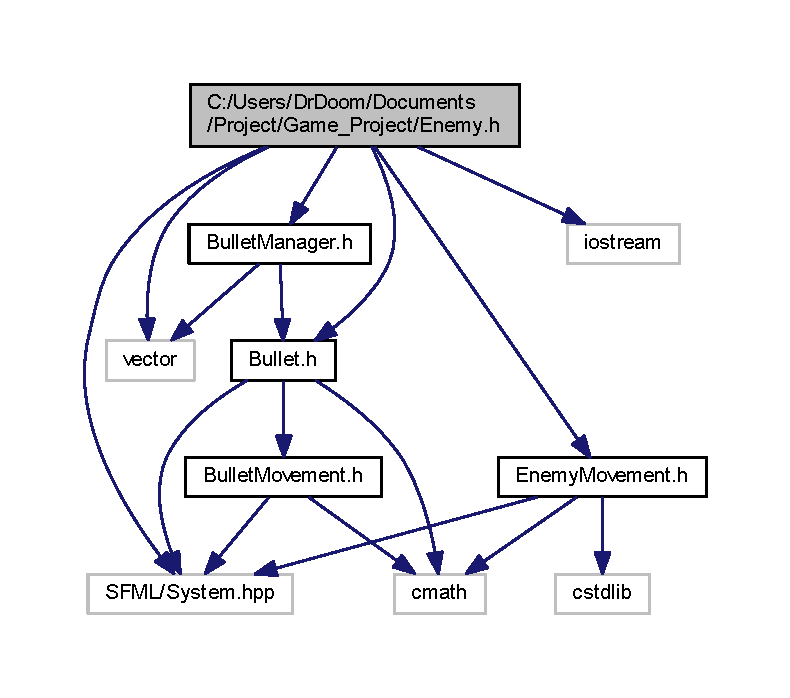
\includegraphics[width=324pt]{_enemy_8h__incl}
\end{center}
\end{figure}
\subsection*{Classes}
\begin{DoxyCompactItemize}
\item 
class \hyperlink{classenemy___file_not_found}{enemy\+\_\+\+File\+Not\+Found}
\item 
class \hyperlink{class_enemy}{Enemy}
\end{DoxyCompactItemize}
\subsection*{Macros}
\begin{DoxyCompactItemize}
\item 
\#define \hyperlink{_enemy_8h_a598a3330b3c21701223ee0ca14316eca}{PI}~3.\+14
\end{DoxyCompactItemize}
\subsection*{Enumerations}
\begin{DoxyCompactItemize}
\item 
enum \hyperlink{_enemy_8h_ac3e413a86119db4b031458c7259e268e}{Enemy\+Type} \{ \hyperlink{_enemy_8h_ac3e413a86119db4b031458c7259e268eaa171194925053f44024a82de9d20148a}{Enemy\+Type\+::\+S\+C\+O\+UT}, 
\hyperlink{_enemy_8h_ac3e413a86119db4b031458c7259e268ea36101183b0be7bffbbe6d24ef81987a1}{Enemy\+Type\+::\+S\+O\+L\+D\+I\+ER}, 
\hyperlink{_enemy_8h_ac3e413a86119db4b031458c7259e268ea416f104f4dfca42fccfd1d6e7534d3ad}{Enemy\+Type\+::\+R\+O\+G\+UE}, 
\hyperlink{_enemy_8h_ac3e413a86119db4b031458c7259e268eafce7f36275b432d29255606c0f395dcd}{Enemy\+Type\+::\+T\+A\+NK}
 \}
\end{DoxyCompactItemize}


\subsection{Detailed Description}
\hyperlink{class_enemy}{Enemy} class, which has 4 types of enemies. Each enemy has a postion, sprite, speed, rotation, bullet damage and the amount of steps taken. The enemy is moved based on its current type. 



\subsection{Macro Definition Documentation}
\mbox{\Hypertarget{_enemy_8h_a598a3330b3c21701223ee0ca14316eca}\label{_enemy_8h_a598a3330b3c21701223ee0ca14316eca}} 
\index{Enemy.\+h@{Enemy.\+h}!PI@{PI}}
\index{PI@{PI}!Enemy.\+h@{Enemy.\+h}}
\subsubsection{\texorpdfstring{PI}{PI}}
{\footnotesize\ttfamily \#define PI~3.\+14}



\subsection{Enumeration Type Documentation}
\mbox{\Hypertarget{_enemy_8h_ac3e413a86119db4b031458c7259e268e}\label{_enemy_8h_ac3e413a86119db4b031458c7259e268e}} 
\index{Enemy.\+h@{Enemy.\+h}!Enemy\+Type@{Enemy\+Type}}
\index{Enemy\+Type@{Enemy\+Type}!Enemy.\+h@{Enemy.\+h}}
\subsubsection{\texorpdfstring{Enemy\+Type}{EnemyType}}
{\footnotesize\ttfamily enum \hyperlink{_enemy_8h_ac3e413a86119db4b031458c7259e268e}{Enemy\+Type}\hspace{0.3cm}{\ttfamily [strong]}}

\begin{DoxyEnumFields}{Enumerator}
\raisebox{\heightof{T}}[0pt][0pt]{\index{S\+C\+O\+UT@{S\+C\+O\+UT}!Enemy.\+h@{Enemy.\+h}}\index{Enemy.\+h@{Enemy.\+h}!S\+C\+O\+UT@{S\+C\+O\+UT}}}\mbox{\Hypertarget{_enemy_8h_ac3e413a86119db4b031458c7259e268eaa171194925053f44024a82de9d20148a}\label{_enemy_8h_ac3e413a86119db4b031458c7259e268eaa171194925053f44024a82de9d20148a}} 
S\+C\+O\+UT&\\
\hline

\raisebox{\heightof{T}}[0pt][0pt]{\index{S\+O\+L\+D\+I\+ER@{S\+O\+L\+D\+I\+ER}!Enemy.\+h@{Enemy.\+h}}\index{Enemy.\+h@{Enemy.\+h}!S\+O\+L\+D\+I\+ER@{S\+O\+L\+D\+I\+ER}}}\mbox{\Hypertarget{_enemy_8h_ac3e413a86119db4b031458c7259e268ea36101183b0be7bffbbe6d24ef81987a1}\label{_enemy_8h_ac3e413a86119db4b031458c7259e268ea36101183b0be7bffbbe6d24ef81987a1}} 
S\+O\+L\+D\+I\+ER&\\
\hline

\raisebox{\heightof{T}}[0pt][0pt]{\index{R\+O\+G\+UE@{R\+O\+G\+UE}!Enemy.\+h@{Enemy.\+h}}\index{Enemy.\+h@{Enemy.\+h}!R\+O\+G\+UE@{R\+O\+G\+UE}}}\mbox{\Hypertarget{_enemy_8h_ac3e413a86119db4b031458c7259e268ea416f104f4dfca42fccfd1d6e7534d3ad}\label{_enemy_8h_ac3e413a86119db4b031458c7259e268ea416f104f4dfca42fccfd1d6e7534d3ad}} 
R\+O\+G\+UE&\\
\hline

\raisebox{\heightof{T}}[0pt][0pt]{\index{T\+A\+NK@{T\+A\+NK}!Enemy.\+h@{Enemy.\+h}}\index{Enemy.\+h@{Enemy.\+h}!T\+A\+NK@{T\+A\+NK}}}\mbox{\Hypertarget{_enemy_8h_ac3e413a86119db4b031458c7259e268eafce7f36275b432d29255606c0f395dcd}\label{_enemy_8h_ac3e413a86119db4b031458c7259e268eafce7f36275b432d29255606c0f395dcd}} 
T\+A\+NK&\\
\hline

\end{DoxyEnumFields}

\hypertarget{_enemy_manager_8h}{}\section{Enemy\+Manager.\+h File Reference}
\label{_enemy_manager_8h}\index{Enemy\+Manager.\+h@{Enemy\+Manager.\+h}}


Manager class for an enemy. This class will maintain the amount of enemies in the game, the enemy\textquotesingle{}s bullets, and the enemy\textquotesingle{}s bullets to the player.  


{\ttfamily \#include $<$vector$>$}\newline
{\ttfamily \#include $<$S\+F\+M\+L/\+System.\+hpp$>$}\newline
{\ttfamily \#include \char`\"{}Enemy.\+h\char`\"{}}\newline
{\ttfamily \#include \char`\"{}Enemy\+Movement.\+h\char`\"{}}\newline
{\ttfamily \#include \char`\"{}Bullet\+Manager.\+h\char`\"{}}\newline
{\ttfamily \#include \char`\"{}Collisions.\+h\char`\"{}}\newline
Include dependency graph for Enemy\+Manager.\+h\+:
% FIG 0
This graph shows which files directly or indirectly include this file\+:
% FIG 1
\subsection*{Classes}
\begin{DoxyCompactItemize}
\item 
class \hyperlink{class_enemy_manager}{Enemy\+Manager}
\end{DoxyCompactItemize}


\subsection{Detailed Description}
Manager class for an enemy. This class will maintain the amount of enemies in the game, the enemy\textquotesingle{}s bullets, and the enemy\textquotesingle{}s bullets to the player. 


\hypertarget{_enemy_movement_8h}{}\section{C\+:/\+Users/\+Dr\+Doom/\+Documents/\+Project/\+Game\+\_\+\+Project/\+Enemy\+Movement.h File Reference}
\label{_enemy_movement_8h}\index{C\+:/\+Users/\+Dr\+Doom/\+Documents/\+Project/\+Game\+\_\+\+Project/\+Enemy\+Movement.\+h@{C\+:/\+Users/\+Dr\+Doom/\+Documents/\+Project/\+Game\+\_\+\+Project/\+Enemy\+Movement.\+h}}


This will move a specific enemy, based on it\textquotesingle{}s type.  


{\ttfamily \#include $<$cstdlib$>$}\newline
{\ttfamily \#include $<$S\+F\+M\+L/\+System.\+hpp$>$}\newline
{\ttfamily \#include $<$cmath$>$}\newline
\subsection*{Classes}
\begin{DoxyCompactItemize}
\item 
class \hyperlink{class_enemy_movement}{Enemy\+Movement}
\end{DoxyCompactItemize}


\subsection{Detailed Description}
This will move a specific enemy, based on it\textquotesingle{}s type. 


\hypertarget{_engine_8h}{}\section{C\+:/\+Users/\+James\+Laptop/\+Documents/\+Default/\+Game\+\_\+\+Project/\+Engine.h File Reference}
\label{_engine_8h}\index{C\+:/\+Users/\+James\+Laptop/\+Documents/\+Default/\+Game\+\_\+\+Project/\+Engine.\+h@{C\+:/\+Users/\+James\+Laptop/\+Documents/\+Default/\+Game\+\_\+\+Project/\+Engine.\+h}}


File Not Found for engine. Used in error catching.  


{\ttfamily \#include $<$S\+F\+M\+L/\+Graphics.\+hpp$>$}\newline
{\ttfamily \#include \char`\"{}Game\+Music.\+h\char`\"{}}\newline
{\ttfamily \#include \char`\"{}Player\+Manager.\+h\char`\"{}}\newline
{\ttfamily \#include \char`\"{}Enemy\+Manager.\+h\char`\"{}}\newline
{\ttfamily \#include \char`\"{}Level.\+h\char`\"{}}\newline
\subsection*{Classes}
\begin{DoxyCompactItemize}
\item 
class \hyperlink{class_file_not_found}{File\+Not\+Found}
\item 
class \hyperlink{class_engine}{Engine}
\end{DoxyCompactItemize}
\subsection*{Enumerations}
\begin{DoxyCompactItemize}
\item 
enum \hyperlink{_engine_8h_a9f5ff9109158e83287c5c888bf7bb8a7}{Screen\+Type} \{ {\bfseries S\+P\+L\+A\+SH}, 
{\bfseries W\+IN}, 
{\bfseries L\+O\+SE}
 \}
\end{DoxyCompactItemize}


\subsection{Detailed Description}
File Not Found for engine. Used in error catching. 

The engine is an instance of the game itself. The engine is the interface to the player, with the play window and player input.

\subsection{Enumeration Type Documentation}
\mbox{\Hypertarget{_engine_8h_a9f5ff9109158e83287c5c888bf7bb8a7}\label{_engine_8h_a9f5ff9109158e83287c5c888bf7bb8a7}} 
\index{Engine.\+h@{Engine.\+h}!Screen\+Type@{Screen\+Type}}
\index{Screen\+Type@{Screen\+Type}!Engine.\+h@{Engine.\+h}}
\subsubsection{\texorpdfstring{Screen\+Type}{ScreenType}}
{\footnotesize\ttfamily enum \hyperlink{_engine_8h_a9f5ff9109158e83287c5c888bf7bb8a7}{Screen\+Type}\hspace{0.3cm}{\ttfamily [strong]}}

An enum for the type of splash screen to be displayed 
\hypertarget{_game_music_8h}{}\section{C\+:/\+Users/\+James\+Laptop/\+Documents/\+Default/\+Game\+\_\+\+Project/\+Game\+Music.h File Reference}
\label{_game_music_8h}\index{C\+:/\+Users/\+James\+Laptop/\+Documents/\+Default/\+Game\+\_\+\+Project/\+Game\+Music.\+h@{C\+:/\+Users/\+James\+Laptop/\+Documents/\+Default/\+Game\+\_\+\+Project/\+Game\+Music.\+h}}


The background music for the game. This class adds for extra functionality than the S\+F\+ML music library, such as pause.  


{\ttfamily \#include $<$S\+F\+M\+L/\+Audio.\+hpp$>$}\newline
\subsection*{Classes}
\begin{DoxyCompactItemize}
\item 
class \hyperlink{class_music___file_not_found}{Music\+\_\+\+File\+Not\+Found}
\item 
class \hyperlink{class_game_music}{Game\+Music}
\end{DoxyCompactItemize}


\subsection{Detailed Description}
The background music for the game. This class adds for extra functionality than the S\+F\+ML music library, such as pause. 


\hypertarget{_level_8h}{}\section{C\+:/\+Users/\+Dr\+Doom/\+Documents/\+Project/\+Game\+\_\+\+Project/\+Level.h File Reference}
\label{_level_8h}\index{C\+:/\+Users/\+Dr\+Doom/\+Documents/\+Project/\+Game\+\_\+\+Project/\+Level.\+h@{C\+:/\+Users/\+Dr\+Doom/\+Documents/\+Project/\+Game\+\_\+\+Project/\+Level.\+h}}


File Not Found for \hyperlink{class_level}{Level}. Used in error catching.  


{\ttfamily \#include $<$S\+F\+M\+L/\+Graphics.\+hpp$>$}\newline
{\ttfamily \#include $<$sstream$>$}\newline
{\ttfamily \#include $<$string$>$}\newline
\subsection*{Classes}
\begin{DoxyCompactItemize}
\item 
class \hyperlink{classlevel___file_not_found}{level\+\_\+\+File\+Not\+Found}
\item 
class \hyperlink{class_level}{Level}
\end{DoxyCompactItemize}


\subsection{Detailed Description}
File Not Found for \hyperlink{class_level}{Level}. Used in error catching. 

The levels for the game as an integer type, up to a certain maximum level.
\hypertarget{_player_8h}{}\section{C\+:/\+Users/\+Dr\+Doom/\+Documents/\+Project/\+Game\+\_\+\+Project/\+Player.h File Reference}
\label{_player_8h}\index{C\+:/\+Users/\+Dr\+Doom/\+Documents/\+Project/\+Game\+\_\+\+Project/\+Player.\+h@{C\+:/\+Users/\+Dr\+Doom/\+Documents/\+Project/\+Game\+\_\+\+Project/\+Player.\+h}}


\hyperlink{class_player}{Player} class has the needed member functions for the player, such as their position, sprite, speed, rotation and their bullets active on the screen. The player\textquotesingle{}s movement is determined by the current input. T\+He player is able to shoot as well.  


{\ttfamily \#include $<$vector$>$}\newline
{\ttfamily \#include $<$S\+F\+M\+L/\+System.\+hpp$>$}\newline
{\ttfamily \#include \char`\"{}Bullet.\+h\char`\"{}}\newline
{\ttfamily \#include \char`\"{}Bullet\+Manager.\+h\char`\"{}}\newline
{\ttfamily \#include \char`\"{}Player\+Movement.\+h\char`\"{}}\newline
{\ttfamily \#include $<$cmath$>$}\newline
\subsection*{Classes}
\begin{DoxyCompactItemize}
\item 
class \hyperlink{classplayer___file_not_found}{player\+\_\+\+File\+Not\+Found}
\item 
class \hyperlink{class_player}{Player}
\end{DoxyCompactItemize}
\subsection*{Macros}
\begin{DoxyCompactItemize}
\item 
\mbox{\Hypertarget{_player_8h_a598a3330b3c21701223ee0ca14316eca}\label{_player_8h_a598a3330b3c21701223ee0ca14316eca}} 
\#define {\bfseries PI}~3.\+14
\end{DoxyCompactItemize}


\subsection{Detailed Description}
\hyperlink{class_player}{Player} class has the needed member functions for the player, such as their position, sprite, speed, rotation and their bullets active on the screen. The player\textquotesingle{}s movement is determined by the current input. T\+He player is able to shoot as well. 


\hypertarget{_player_manager_8h}{}\section{C\+:/\+Users/\+James\+Laptop/\+Documents/\+Default/\+Game\+\_\+\+Project/\+Player\+Manager.h File Reference}
\label{_player_manager_8h}\index{C\+:/\+Users/\+James\+Laptop/\+Documents/\+Default/\+Game\+\_\+\+Project/\+Player\+Manager.\+h@{C\+:/\+Users/\+James\+Laptop/\+Documents/\+Default/\+Game\+\_\+\+Project/\+Player\+Manager.\+h}}


The playermanager will maintain all updates and events to the player, such as player input, collision detection, drawing the player to the active window.  


{\ttfamily \#include \char`\"{}Player.\+h\char`\"{}}\newline
{\ttfamily \#include \char`\"{}Collisions.\+h\char`\"{}}\newline
{\ttfamily \#include $<$vector$>$}\newline
{\ttfamily \#include $<$S\+F\+M\+L/\+System.\+hpp$>$}\newline
{\ttfamily \#include $<$sstream$>$}\newline
\subsection*{Classes}
\begin{DoxyCompactItemize}
\item 
class \hyperlink{class_player_manager}{Player\+Manager}
\end{DoxyCompactItemize}
\subsection*{Enumerations}
\begin{DoxyCompactItemize}
\item 
enum \hyperlink{_player_manager_8h_a00ec4eba48da32d6cbdf827185fd3d34}{Move\+Direction} \{ {\bfseries R\+I\+G\+HT}, 
{\bfseries L\+E\+FT}, 
{\bfseries S\+T\+O\+P\+\_\+\+R\+I\+G\+HT}, 
{\bfseries S\+T\+O\+P\+\_\+\+L\+E\+FT}
 \}
\end{DoxyCompactItemize}


\subsection{Detailed Description}
The playermanager will maintain all updates and events to the player, such as player input, collision detection, drawing the player to the active window. 



\subsection{Enumeration Type Documentation}
\mbox{\Hypertarget{_player_manager_8h_a00ec4eba48da32d6cbdf827185fd3d34}\label{_player_manager_8h_a00ec4eba48da32d6cbdf827185fd3d34}} 
\index{Player\+Manager.\+h@{Player\+Manager.\+h}!Move\+Direction@{Move\+Direction}}
\index{Move\+Direction@{Move\+Direction}!Player\+Manager.\+h@{Player\+Manager.\+h}}
\subsubsection{\texorpdfstring{Move\+Direction}{MoveDirection}}
{\footnotesize\ttfamily enum \hyperlink{_player_manager_8h_a00ec4eba48da32d6cbdf827185fd3d34}{Move\+Direction}\hspace{0.3cm}{\ttfamily [strong]}}

An enum for the direction of movement of the player 
\hypertarget{_player_movement_8h}{}\section{C\+:/\+Users/\+Dr\+Doom/\+Documents/\+Project/\+Game\+\_\+\+Project -\/ Copy/\+Player\+Movement.h File Reference}
\label{_player_movement_8h}\index{C\+:/\+Users/\+Dr\+Doom/\+Documents/\+Project/\+Game\+\_\+\+Project -\/ Copy/\+Player\+Movement.\+h@{C\+:/\+Users/\+Dr\+Doom/\+Documents/\+Project/\+Game\+\_\+\+Project -\/ Copy/\+Player\+Movement.\+h}}


The movement of the player. The player will either move clockwise or counter clockwise along the radial path.  


\subsection*{Classes}
\begin{DoxyCompactItemize}
\item 
class \hyperlink{class_player_movement}{Player\+Movement}
\end{DoxyCompactItemize}


\subsection{Detailed Description}
The movement of the player. The player will either move clockwise or counter clockwise along the radial path. 


%--- End generated contents ---

% Index
\backmatter
\newpage
\phantomsection
\clearemptydoublepage
\addcontentsline{toc}{chapter}{Index}
\printindex

\end{document}
